\documentclass[11pt,letterpaper,openany]{report}

\usepackage[letterpaper,top=0.78in,bottom=0.82in,left=0.82in,right=0.82in,headheight=15pt]{geometry}
\usepackage{fontspec}
\usepackage{graphicx}
\setmainfont{TeXGyrePagella}
\setsansfont{Inter}
\setmonofont{DejaVu Sans Mono}[Scale=0.82]
\usepackage{microtype}
\usepackage[table]{xcolor}
\usepackage{amsmath,amssymb,mathtools}
\usepackage{array,booktabs,longtable,tabularx,multirow}
\usepackage{enumitem}
\usepackage{listings}
\usepackage{upquote}
\usepackage{xurl}
\usepackage{hyperref}
\usepackage{bookmark}
\usepackage[capitalise,noabbrev]{cleveref}
\usepackage{fancyhdr}
\usepackage{titlesec}
\usepackage{tikz}
\usetikzlibrary{arrows.meta,positioning,fit,calc,backgrounds,shapes.multipart}
\usepackage[most]{tcolorbox}
\usepackage{ragged2e}
\usepackage{caption}
\usepackage{float}

\definecolor{Ink}{HTML}{17212B}
\definecolor{Slate}{HTML}{52606D}
\definecolor{Accent}{HTML}{22577A}
\definecolor{AccentLight}{HTML}{E8F1F6}
\definecolor{Green}{HTML}{2D6A4F}
\definecolor{GreenLight}{HTML}{EAF4EF}
\definecolor{Gold}{HTML}{8A5A00}
\definecolor{GoldLight}{HTML}{FFF5DA}
\definecolor{Red}{HTML}{9B2226}
\definecolor{RedLight}{HTML}{FCEBEC}
\definecolor{Purple}{HTML}{5B3F8C}
\definecolor{PurpleLight}{HTML}{F0EBF8}
\definecolor{CodeBg}{HTML}{F5F7F9}
\definecolor{CodeRule}{HTML}{D5DCE3}

\hypersetup{
  colorlinks=true,
  linkcolor=Accent,
  urlcolor=Accent,
  citecolor=Green,
  hypertexnames=false,
  pdftitle={Proof-Producing Automation for Lean 4},
  pdfauthor={OpenAI},
  pdfsubject={Integrating Leant/Djex, Z3, and Lean's native solver infrastructure},
  pdfkeywords={Lean 4, Leant, Djex, Djinn, Exference, Z3, SMT, grind, proof automation, synthesis, certificates}
}

\pagestyle{fancy}
\fancyhf{}
\fancyhead[L]{\small\sffamily\color{Slate}\nouppercase{\leftmark}}
\fancyhead[R]{\small\sffamily\color{Slate}Lean proof automation}
\fancyfoot[L]{\small\sffamily\color{Slate}10 August 2026}
\fancyfoot[R]{\small\sffamily\color{Slate}\thepage}
\renewcommand{\headrulewidth}{0.35pt}
\renewcommand{\footrulewidth}{0pt}
\fancypagestyle{plain}{%
  \fancyhf{}
  \fancyfoot[C]{\small\sffamily\color{Slate}\thepage}
  \renewcommand{\headrulewidth}{0pt}
}

\titleformat{\chapter}[display]
  {\bfseries\sffamily\color{Ink}}
  {\filleft\Large\color{Accent}\chaptertitlename\ \thechapter}
  {1ex}
  {\titlerule\vspace{1.1ex}\Huge}
\titleformat{\section}
  {\Large\bfseries\sffamily\color{Ink}}{\thesection}{0.65em}{}
\titleformat{\subsection}
  {\large\bfseries\sffamily\color{Ink}}{\thesubsection}{0.6em}{}
\titleformat{\subsubsection}
  {\normalsize\bfseries\sffamily\color{Ink}}{\thesubsubsection}{0.55em}{}
\titlespacing*{\chapter}{0pt}{-18pt}{24pt}
\titlespacing*{\section}{0pt}{2.1ex plus .7ex minus .2ex}{0.9ex}
\titlespacing*{\subsection}{0pt}{1.7ex plus .5ex minus .2ex}{0.65ex}

\setcounter{tocdepth}{2}
\setcounter{secnumdepth}{3}
\setlist[itemize]{leftmargin=1.42em,itemsep=0.24em,topsep=0.38em}
\setlist[enumerate]{leftmargin=1.7em,itemsep=0.27em,topsep=0.4em}
\setlength{\parindent}{0pt}
\setlength{\parskip}{0.52em}
\setlength{\emergencystretch}{3em}
\renewcommand{\arraystretch}{1.16}
\captionsetup{font=small,labelfont=bf}

\lstdefinelanguage{LeanFour}{
  morekeywords={namespace,end,inductive,structure,def,theorem,lemma,where,match,with,if,then,else,let,in,fun,forall,Prop,Type,Sort,variable,deriving,instance,class,private,public,partial,unsafe,opaque,axiom,example,by,have,show,from,return,do,try,catch,throw,exact,refine,apply,intro,cases,induction,constructor,simp,grind,omega,noncomputable,set_option,import,open,elab,syntax,macro,run_tac},
  sensitive=true,
  morecomment=[l]{--},
  morecomment=[s]{/-}{-/},
  morestring=[b]"
}
\lstdefinelanguage{HaskellLite}{
  morekeywords={data,type,newtype,class,instance,where,deriving,module,import,qualified,as,case,of,let,in,do,if,then,else,otherwise,forall,pattern},
  sensitive=true,
  morecomment=[l]{--},
  morecomment=[s]{\{-}{-\}},
  morestring=[b]"
}
\lstdefinelanguage{SMTLIB}{
  morekeywords={set-logic,set-option,declare-sort,declare-fun,declare-const,define-fun,define-fun-rec,assert,check-sat,check-sat-assuming,get-model,get-value,get-unsat-core,get-proof,get-info,push,pop,echo,forall,exists,let,ite,match,as,par,Int,Real,Bool,Array,Seq,BitVec,minimize,maximize},
  sensitive=true,
  morecomment=[l]{;},
  morestring=[b]"
}
\lstdefinelanguage{JSONLite}{
  morestring=[b]",
  morecomment=[l]{//},
  literate=
   *{0}{{{\color{Purple}0}}}{1}
    {1}{{{\color{Purple}1}}}{1}
    {2}{{{\color{Purple}2}}}{1}
    {3}{{{\color{Purple}3}}}{1}
    {4}{{{\color{Purple}4}}}{1}
    {5}{{{\color{Purple}5}}}{1}
    {6}{{{\color{Purple}6}}}{1}
    {7}{{{\color{Purple}7}}}{1}
    {8}{{{\color{Purple}8}}}{1}
    {9}{{{\color{Purple}9}}}{1}
}
\lstset{
  basicstyle=\ttfamily\small,
  backgroundcolor=\color{CodeBg},
  rulecolor=\color{CodeRule},
  frame=single,
  framerule=0.35pt,
  framesep=5pt,
  xleftmargin=0.35em,
  xrightmargin=0.35em,
  breaklines=true,
  breakatwhitespace=false,
  showstringspaces=false,
  columns=fullflexible,
  keepspaces=true,
  tabsize=2,
  keywordstyle=\bfseries\color{Accent},
  commentstyle=\itshape\color{Green},
  stringstyle=\color{Gold},
  aboveskip=0.75em,
  belowskip=0.75em
}

\newtcolorbox{keybox}[1][]{
  enhanced,colback=AccentLight,colframe=Accent,boxrule=0.7pt,arc=2pt,
  left=8pt,right=8pt,top=7pt,bottom=7pt,fonttitle=\bfseries\sffamily,#1
}
\newtcolorbox{soundbox}[1][]{
  enhanced,colback=GreenLight,colframe=Green,boxrule=0.7pt,arc=2pt,
  left=8pt,right=8pt,top=7pt,bottom=7pt,fonttitle=\bfseries\sffamily,#1
}
\newtcolorbox{warningbox}[1][]{
  enhanced,colback=GoldLight,colframe=Gold,boxrule=0.7pt,arc=2pt,
  left=8pt,right=8pt,top=7pt,bottom=7pt,fonttitle=\bfseries\sffamily,#1
}
\newtcolorbox{riskbox}[1][]{
  enhanced,colback=RedLight,colframe=Red,boxrule=0.7pt,arc=2pt,
  left=8pt,right=8pt,top=7pt,bottom=7pt,fonttitle=\bfseries\sffamily,#1
}
\newtcolorbox{designbox}[1][]{
  enhanced,colback=PurpleLight,colframe=Purple,boxrule=0.7pt,arc=2pt,
  left=8pt,right=8pt,top=7pt,bottom=7pt,fonttitle=\bfseries\sffamily,#1
}

\newcolumntype{Y}{>{\RaggedRight\arraybackslash}X}
\newcolumntype{L}[1]{>{\RaggedRight\arraybackslash}p{#1}}
\newcommand{\Lean}{\textsc{Lean 4}}
\newcommand{\Leant}{\textsc{Leant}}
\newcommand{\Djex}{\textsc{Djex}}
\newcommand{\Djinn}{\textsc{Djinn}}
\newcommand{\Exference}{\textsc{Exference}}
\newcommand{\Zthree}{\textsc{Z3}}
\newcommand{\code}[1]{\texttt{\detokenize{#1}}}
\newcommand{\filepath}[1]{\nolinkurl{#1}}
\newcommand{\repo}[1]{\textsf{#1}}
\newcommand{\commit}[1]{\texttt{\small #1}}
\newcommand{\sourcelink}[2]{\href{#1}{\nolinkurl{#2}}}
\newcommand{\priohigh}{\textcolor{Green}{\textbf{strong}}}
\newcommand{\priomed}{\textcolor{Gold}{\textbf{medium}}}
\newcommand{\priolow}{\textcolor{Red}{\textbf{weak}}}
\newcommand{\priodefer}{\textcolor{Purple}{\textbf{defer}}}
\newcommand{\yes}{\textcolor{Green}{\textbf{yes}}}
\newcommand{\partialyes}{\textcolor{Gold}{\textbf{partial}}}
\newcommand{\no}{\textcolor{Red}{\textbf{no}}}

\begin{document}
\hypersetup{pageanchor=false}
\pagenumbering{gobble}

\begin{titlepage}
  \thispagestyle{empty}
  \vspace*{10mm}
  {\sffamily\bfseries\fontsize{29}{34}\selectfont\color{Ink}
    Proof-Producing Automation\\[2mm]
    for Lean 4\par}
  \vspace{5mm}
  {\sffamily\fontsize{18}{23}\selectfont\color{Accent}
    Integrating Leant/Djex, Z3, and Lean's native solver infrastructure\par}
  \vspace{13mm}

  \begin{keybox}[title=Central conclusion]
  The most promising architecture is not to trust an external solver and not to
  replace Lean's tactics. It is a proof-producing portfolio: Leant/Djex proposes
  typed structural proof skeletons; Z3 supplies semantic countermodels, unsat
  cores, quantifier instances, and synthesized parameters; Lean reconstructs a
  proof from those hints or checks a small certificate; and the kernel remains the
  sole acceptance boundary.
  \end{keybox}

  \vfill
  \begin{tabular}{@{}ll@{}}
    \textsf{Prepared for:} & Vladimir Reshetnikov \\
    \textsf{Date:} & 10 August 2026 \\
    \textsf{Primary repositories:} & \repo{leanprover/lean4} \\
                                  & \repo{Z3Prover/z3} \\
                                  & \repo{VladimirReshetnikov/Leant} \\
    \textsf{Related pinned component:} & \repo{VladimirReshetnikov/Djex}
  \end{tabular}
  \vspace{11mm}

  {\small\color{Slate}
  The analysis is pinned to exact commits in \cref{ch:scope}. The report is an
  architectural and implementation feasibility study; it does not claim that the
  proposed tactics or protocols have already been implemented.}
\end{titlepage}

\hypersetup{pageanchor=true}
\pagenumbering{roman}

\chapter*{Abstract}
\addcontentsline{toc}{chapter}{Abstract}
Lean 4 already contains the ingredients of a modern proof-producing automation
platform: an extensible elaborator and metaprogramming layer; a backtrackable,
proof-reconstructing congruence and E-matching engine in \code{grind}; replayable
editor suggestions through \code{TryThis}; a pluggable library-premise selector;
specialized arithmetic solvers; and a reflected bit-vector tactic whose external
SAT result is accepted only after an LRAT certificate is checked in Lean. Recent
work has also begun to let tactics share \code{grind}'s normalized state instead of
operating as isolated black boxes.

Leant and its pinned Djex engine contribute a complementary capability. They search
for Curry--Howard inhabitants rather than merely deciding a first-order formula.
Djinn performs bounded but complete structural proof search on its admitted
intuitionistic fragment and can distinguish a genuine refutation from bounded
failure. Exference performs ranked heuristic synthesis. Leant serializes a
substantial fragment of an elaborated Lean target, discovers bounded exact provider
metadata from the active environment, renders candidates, and then re-elaborates
every candidate as a temporary Lean example. This is already a strong untrusted-
generator/trusted-checker arrangement. Its limitations are mainly representational:
the current public result is rendered source text rather than a typed proof graph,
proof search is exposed through a separate REPL rather than a native tactic, and a
successful candidate is generally all-or-nothing rather than a skeleton with typed
residual goals.

Z3 contributes strong semantic search over quantifier-free and quantified
first-order theories, models, assumption-based unsat cores, optimization,
fixedpoint/Horn solving, model-based projection, and configurable proof logging. Its
outputs have different logical strengths. A model after \code{sat} can support a
counterexample only when the encoding and decoder are validated. An unsat core is a
premise-selection hint, not a proof. A raw Z3 proof object or self-validated inference
log is not automatically an independently checked Lean certificate. A result of
\code{unknown} must remain explicit; a model returned after \code{unknown} is not, in
general, a valid counterexample. These distinctions should be represented in the API
rather than buried in diagnostic strings.

The recommended system is a layered portfolio. A Lean-side goal snapshot and
projection layer assigns stable identities to binders, constants, theorem premises,
and source occurrences. Untrusted workers then contribute different artifacts:
Leant/Djex supplies typed proof graphs and hole-bearing structural skeletons; Z3
supplies validated finite models, unsat cores, candidate instantiations, arithmetic
coefficients, invariants, and branch-feasibility results; Lean-native tactics supply
proof-producing normalization and decision procedures. A reconstruction layer turns
all proof-bearing artifacts into Lean expressions or tactic scripts and leaves every
unsupported step as an ordinary residual goal. Only kernel-accepted terms close a
goal. Diagnostic artifacts are shown with weaker result labels and never silently
promoted to proofs.

The report proposes concrete Lean and wire-level data structures, a native
\code{leant?}/\code{leant} tactic, a typed proof-skeleton protocol, a staged
\code{z3?} oracle, theory-specific reconstruction for EUF, linear arithmetic, bit
vectors, arrays, and algebraic datatypes, cooperation with \code{grind} and
\code{LibrarySuggestions}, counterexample-guided synthesis, induction and invariant
synthesis, proof repair, deterministic scheduling, caching, process isolation, and a
benchmark methodology. The highest-value first implementation is deliberately
modest: expose Leant as a native suggestion tactic, retain current Lean
re-elaboration as the acceptance boundary, and add typed holes before attempting a
generic Z3 proof-object checker.

\tableofcontents
\clearpage
\pagenumbering{arabic}

\chapter{Executive conclusions}
\label{ch:executive}

\section{Bottom line}

\begin{keybox}[title=Primary recommendation]
Build a single proof-automation portfolio around a typed, source-mapped proof graph.
Use Leant/Djex for structural proof construction, Z3 for semantic search and
counterexample generation, and Lean's existing tactics for normalization and proof
reconstruction. Treat every external component as an untrusted producer of
candidates or evidence. The only operation that closes a goal is construction of a
Lean term accepted by the current elaborator and kernel, or execution of a small
certificate checker whose soundness theorem is itself kernel-checked.
\end{keybox}

This division of labor matches the actual strengths of the three codebases:

\begin{itemize}
  \item \textbf{Lean knows the exact dependent type theory, elaboration state, local
        instances, coercions, reducibility settings, universe constraints, and source
        context.} It should own projection, reconstruction, and final checking.
  \item \textbf{Leant/Djex knows how to construct inhabitants.} It is especially useful
        for introductions, higher-order use of hypotheses and providers, constructor
        and case structure, rank-N instantiation within explicit bounds, and short
        compositions that are awkward for first-order SMT encodings.
  \item \textbf{Z3 knows how to search semantic spaces.} It is especially useful for
        finding countermodels, eliminating impossible branches, selecting a small set
        of premises, proposing quantifier instances, solving arithmetic templates,
        minimizing choices, and synthesizing invariants or ranking parameters.
  \item \textbf{Lean's native solvers know how to turn many of those facts into proofs.}
        \code{grind}, \code{omega}/linear-arithmetic extensions,
        \code{grobner}, simplification, congruence closure, and \code{bv_decide}
        already produce or check proof evidence in the target system.
\end{itemize}

The architecture should therefore optimize the exchange of \emph{typed hints} rather
than search for one universal solver.

\section{The seven most valuable directions}

\begin{longtable}{@{}L{0.19\textwidth}L{0.29\textwidth}L{0.25\textwidth}L{0.17\textwidth}@{}}
\toprule
\textbf{Direction} & \textbf{What it adds} & \textbf{Soundness path} & \textbf{Priority} \\
\midrule
\endhead
Native \code{leant?}/\code{leant} tactic & Makes structural synthesis available at any Lean goal; emits a pasteable proof suggestion. & Re-elaborate candidate in the saved tactic state; kernel checks final term. & \priohigh \\
Typed, hole-bearing skeletons & Lets Leant solve introductions, applications, cases, and constructors while leaving arithmetic or domain facts to other tactics. & Reconstruct with \code{refine}; every hole remains a Lean metavariable. & \priohigh \\
Z3 counterexample and core oracle & Gives concrete failures, premise minimization, infeasible branch detection, and better diagnostics before expensive search. & Validate model decoding; treat cores as hints only. & \priohigh \\
Theory-specific proof reconstruction & Converts Z3 discoveries into calls to Lean's EUF, arithmetic, bit-vector, array, and datatype proof infrastructure. & Lean tactic or small checker produces the proof. & \priohigh \\
Cooperative \code{solve?} portfolio & Schedules Lean-native solvers, Leant, premise selection, and Z3 under deterministic budgets. & Each lane has its own evidence label; only checked proofs close. & \priohigh \\
Induction and invariant synthesis & Leant chooses recursors and proof shape; Z3 solves coefficient, invariant, or ranking templates; Lean checks VCs. & Kernel checks base, step, postcondition, and decrease obligations. & \priomed \\
Generic Z3 proof-object translation & Potentially replays a wider SMT proof directly. & Requires a large, version-sensitive parser and independently proved checker. & \priodefer \\
\bottomrule
\end{longtable}

\section{What should not be built first}

Three tempting approaches have a poor cost-to-trust ratio as initial projects.

\begin{enumerate}
  \item \textbf{Do not make \code{unsat} a primitive Lean axiom.} This would enlarge the
        trusted base to include the translator, solver binary, options, theory
        semantics, protocol, and process boundary. It would also make proof replay and
        regression diagnosis much worse.
  \item \textbf{Do not start with a universal Lean-to-SMT translator.} Dependent types,
        type classes, coercions, partial operations, quotients, proof irrelevance,
        recursive definitions, and definitional equality make ``translate everything''
        an endless source of semantic gaps. Begin with exact, named fragments and
        leave residual goals.
  \item \textbf{Do not start by parsing every Z3 proof rule.} Z3's proof support is
        solver-configuration-dependent, broad, and evolving. For the first useful
        system, reconstruct results through Lean's own theory tactics and check small
        certificates such as LRAT where a mature checker already exists.
\end{enumerate}

\begin{soundbox}[title=Positive results are cheap to trust; negative results are not]
A proposed proof term can be completely untrusted: Lean either accepts it at the
exact target or rejects it. By contrast, ``no proof exists'', ``this branch is
impossible'', or ``this model refutes the theorem'' requires a precise projection
contract. The system should preserve that asymmetry explicitly in every result type.
\end{soundbox}

\section{A concrete first result}

The first implementation target should be a package tentatively named
\code{Leant.Tactic} with the following behavior:

\begin{lstlisting}[language=LeanFour,caption={Proposed first user-facing command}]
import Leant.Tactic

example (A B C : Prop)
    (f : A -> B -> C) (g : A -> B) (a : A) : C := by
  leant?
-- Try this:
--   exact f a (g a)
\end{lstlisting}

The initial version may keep the existing Haskell worker and even the current rendered
candidate format. The Lean tactic should snapshot the goal, invoke a revision-pinned
worker, verify each candidate against the saved state, and use \code{TryThis} to show
the first accepted script. That produces immediate value while establishing the
transport, cancellation, stale-result, and test infrastructure needed by every later
feature.

\chapter{Scope, method, and repository snapshots}
\label{ch:scope}

\section{Exact revisions}

The review was performed on 10 August 2026 against the revisions below. The Leant
repository head contains report-only commits after its latest functional integration;
where implementation details are discussed, source links use the latest functional
commit \commit{0160237e4bdf}. Leant's Djex submodule pin was read from the repository
tree rather than inferred from documentation.

\begin{longtable}{@{}L{0.18\textwidth}L{0.25\textwidth}L{0.48\textwidth}@{}}
\toprule
\textbf{Repository} & \textbf{Pinned revision} & \textbf{Relevant state} \\
\midrule
\endhead
\repo{leanprover/lean4} &
\href{https://github.com/leanprover/lean4/tree/1d2dde6d64cb3da989bab118f4d386eb55237fe5}{\commit{1d2dde6d64cb}} &
Current development head at the time of review. Includes the modular \code{grind}
engine, replayable \code{grind?}, library suggestions, symbolic tactic integration,
LRAT-backed \code{bv_decide}, and the recent sharing of \code{grind} state with
\code{bv_decide}. \\
\repo{Z3Prover/z3} &
\href{https://github.com/Z3Prover/z3/tree/0bd679a404bee551393fd94ca813ccc7eb034973}{\commit{0bd679a404be}} &
Current development head. Exposes models, proofs, unsat cores, optimization,
fixedpoint/Horn solving, quantifiers, algebraic datatypes, arrays, sequences,
bit-vectors, and configurable proof logging. \\
\repo{Leant} &
\href{https://github.com/VladimirReshetnikov/Leant/tree/dab7a1518f51faf5e71cb71142c5c4df3904774e}{\commit{dab7a1518f51}} &
Repository head. Latest functional source is represented by
\href{https://github.com/VladimirReshetnikov/Leant/tree/0160237e4bdf6e342a55f5a86ce5d5292728024f}{\commit{0160237e4bdf}},
followed by documentation commits. \\
\repo{Djex} &
\href{https://github.com/VladimirReshetnikov/Djex/tree/f50b5eac86726c7530d95e48c27101b7c0fa25c9}{\commit{f50b5eac8672}} &
Exact Leant submodule pin. Provides the checked Djinn and Exference adapters, common
query/evidence vocabulary, bounded rank-N/provider support, and generated expression
infrastructure. \\
\repo{ufmg-smite/lean-smt} &
\href{https://github.com/ufmg-smite/lean-smt/tree/a4ed29b0b9fd840eefefa33146eb8fa3e14d35da}{\commit{a4ed29b0b9fd}} &
Comparison point: active beta tactic that sends Lean goals to cvc5 and replays solver
proofs in Lean, leaving unsupported proof steps as residual Lean goals. \\
\bottomrule
\end{longtable}

\section{Questions investigated}

The investigation focused on five engineering questions.

\begin{enumerate}
  \item Which current extension points in Lean can host external structural and
        semantic automation without patching the kernel or depending prematurely on
        unstable internals?
  \item Which information does Leant/Djex already preserve, and which information is
        lost when a checked candidate becomes rendered source text?
  \item Which Z3 outputs can safely be used as proofs, proof plans, diagnostics,
        counterexamples, or search heuristics?
  \item How can the systems cooperate on one proof state instead of merely racing as
        independent tactics?
  \item What staged implementation produces useful results while keeping the trusted
        computing base small and every failure mode explicit?
\end{enumerate}

The report is intentionally architecture-oriented. It reviews exact source seams and
recent development direction, but it does not attempt a benchmark run or implement a
prototype. Proposed APIs are schematic and are meant to make data ownership,
verification, and versioning precise; exact names would naturally change during
implementation.

\section{Terminology}

\begin{description}[style=nextline,leftmargin=1.8em]
  \item[Candidate] An untrusted proposed Lean term, tactic script, proof graph, theorem
        instance, model, or solver-derived fact.
  \item[Reconstruction] Building a Lean proof from external hints using elaboration,
        theorem application, native tactics, or a verified checker.
  \item[Certificate] Data checked by a comparatively small Lean program whose
        soundness theorem implies the desired proposition.
  \item[Projection] A controlled translation from an elaborated Lean goal or subgoal
        to another calculus or semantic theory.
  \item[Residual goal] A Lean metavariable intentionally left by a partial proof
        skeleton for another tactic or the user.
  \item[Proof-producing portfolio] A scheduler in which heterogeneous engines may
        search aggressively, but every successful lane returns a kernel-checkable
        proof or checked certificate.
\end{description}

\chapter{Lean 4 as the proof-producing host}
\label{ch:lean}

\section{The relevant architecture is already present}

Lean's current tactic infrastructure is not a thin wrapper over kernel primitives. It
contains a substantial proof-producing search substrate. The most relevant components
are shown in \cref{fig:lean-substrate}.

\begin{figure}[H]
\centering
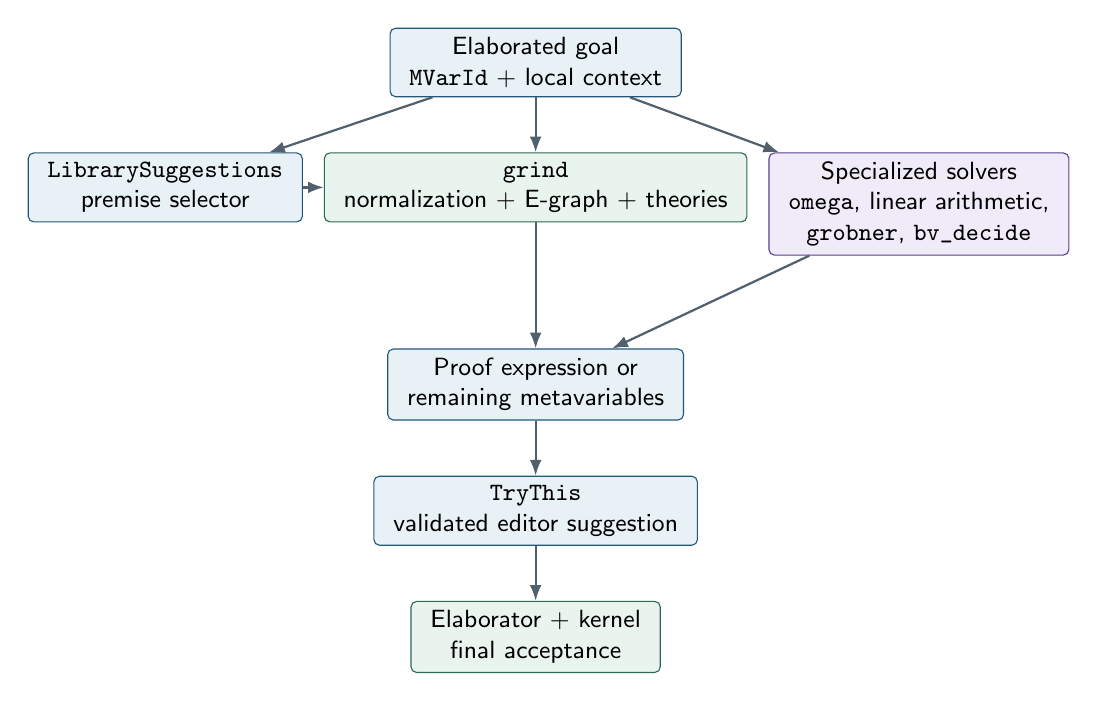
\begin{tikzpicture}[
  node distance=7mm and 11mm,
  every node/.style={font=\small\sffamily},
  box/.style={draw=Accent,rounded corners=2pt,fill=AccentLight,align=center,minimum height=8mm,inner xsep=7pt},
  green/.style={draw=Green,rounded corners=2pt,fill=GreenLight,align=center,minimum height=8mm,inner xsep=7pt},
  purple/.style={draw=Purple,rounded corners=2pt,fill=PurpleLight,align=center,minimum height=8mm,inner xsep=7pt},
  arr/.style={-{Latex[length=2mm]},thick,color=Slate}
]
\node[box] (goal) {Elaborated goal\\\code{MVarId} + local context};
\node[box,below left=of goal] (libs) {\code{LibrarySuggestions}\\premise selector};
\node[green,below=of goal] (grind) {\code{grind}\\normalization + E-graph + theories};
\node[purple,below right=of goal] (spec) {Specialized solvers\\\code{omega}, linear arithmetic,\\\code{grobner}, \code{bv_decide}};
\node[box,below=16mm of grind] (proof) {Proof expression or\\remaining metavariables};
\node[box,below=of proof] (trythis) {\code{TryThis}\\validated editor suggestion};
\node[green,below=of trythis] (kernel) {Elaborator + kernel\\final acceptance};
\draw[arr] (goal) -- (grind);
\draw[arr] (goal) -- (libs);
\draw[arr] (libs) -- (grind);
\draw[arr] (goal) -- (spec);
\draw[arr] (grind) -- (proof);
\draw[arr] (spec) -- (proof);
\draw[arr] (proof) -- (trythis);
\draw[arr] (trythis) -- (kernel);
\end{tikzpicture}
\caption{Lean's existing substrate already separates premise selection, proof search,
specialized decision procedures, validated suggestions, and kernel acceptance.}
\label{fig:lean-substrate}
\end{figure}

This matters because external tools do not need to own the tactic experience. They can
enter at several narrower seams: selecting premises, proposing a proof skeleton,
proposing derived facts, supplying a theory certificate, or generating a diagnostic
model.

\section{\code{grind}: a natural cooperation point}

At the pinned revision, \code{grind} is a modular goal-level engine rather than a
single opaque tactic. Its elaborator builds parameters from explicit theorem patterns,
configuration, and library suggestions. The meta-level engine maintains a
backtrackable state containing simplification data, congruence information, E-matching
theorems and constraints, split sources, diagnostics, theory-solver state, and proof
reconstruction information. Specialized front ends for linear integer arithmetic,
linear arithmetic, order reasoning, and Groebner-style algebra use the same core.

Several details are particularly important for future integration:

\begin{itemize}
  \item E-matching theorems carry origins, proof expressions, patterns, symbols, and
        bounded constraints such as generation, size, depth, groundness, values, and a
        maximum number of instances.
  \item The engine receives an array of extension states. This shows that the
        implementation already thinks in terms of cooperating theory or theorem
        extensions, even though a stable third-party solver-extension API should not be
        assumed from current internal types.
  \item \code{grind?} does not merely print a heuristic recommendation. It constructs a
        self-contained script and validates it through the standard suggestion
        machinery before presenting it.
  \item The elaborator can call \code{LibrarySuggestions.select} with the caller name
        \code{"grind"}, so premise retrieval is already a replaceable component rather
        than hard-coded theorem enumeration.
\end{itemize}

The most informative recent change is the integration of \code{bv_decide} with
interactive \code{grind}. The bit-vector tactic can consume relevant equivalence
classes and learned facts from the current \code{grind} state before bit-blasting.
This is precisely the cooperation pattern a future Z3 or Leant bridge should emulate:
share normalized facts and source identities, then let a specialized solver produce
its own independently checked evidence.

\begin{warningbox}[title=Do not bind the first prototype to private \code{grind} internals]
The \code{grind} implementation is moving quickly. Canonicalization, pattern handling,
homomorphism support, symbolic execution, and theory integration have all changed
recently. The first external integration should be a sibling tactic that exchanges
ordinary Lean facts and residual goals. A true solver extension should follow only
after a stable public interface exists or after the interface is designed together
with Lean maintainers.
\end{warningbox}

\section{\code{TryThis}: the right user-interface seam}

\code{Lean.Meta.Tactic.TryThis} already supports validated editor code actions. It can
save and restore tactic state, check a proposed script, emit \code{exact} or
\code{refine}, insert \code{expose_names} when generated references require stable
names, and preserve remaining subgoals. This makes it an ideal endpoint for external
automation:

\begin{itemize}
  \item \code{leant?} can show a structural term or a \code{refine} skeleton.
  \item \code{z3?} can show a reconstructed proof plan, a minimal set of premises, or a
        counterexample diagnostic without changing the goal.
  \item \code{solve?} can compare candidates from several lanes and present the
        shortest validated script rather than the first raw solver response.
\end{itemize}

A crucial design rule follows: the external protocol should not be responsible for
pretty-printing the final user script. It should return structured references and
proof nodes. Lean should elaborate, normalize names, decide whether \code{exact} or
\code{refine} is appropriate, and then ask \code{TryThis} to validate the final text.

\section{\code{LibrarySuggestions}: premise selection as a first-class service}

The core suggestion API maps a goal and configuration to scored theorem suggestions.
The configuration records the caller, a maximum result count, filters, and an
arbitrary hint. The API also provides combinators for combining and filtering
selectors and utilities for collecting constants and relevant constants from a goal.
No single premise-selection algorithm is privileged.

This is a strong insertion point for both Leant and Z3:

\begin{itemize}
  \item Leant's live provider inventory can be seeded by a selector instead of scanning
        a broad declaration prefix. The engine can still widen geometrically if the
        first ranked providers fail.
  \item A Z3 unsat core can feed back which translated premises were actually needed.
        Repeated results can train or heuristically adjust theorem scores without
        trusting the core as a proof.
  \item Model-based diagnostics can identify which missing relation or constructor
        fact blocks the current proof and request more premises sharing those symbols.
  \item The selector hint can carry a normalized goal signature or feature vector
        without changing the theorem-search API.
\end{itemize}

\section{Reflected checking in \texttt{bv\_decide}}

The current bit-vector tactic is a model for trustworthy external acceleration. It
bit-blasts a reflected bit-vector expression, converts the result to CNF, parses an
LRAT certificate, and runs a Lean checker. The theorem
\code{verifyCert_correct} connects a successful checker result to CNF
unsatisfiability; another theorem connects the bit-blasted CNF back to the original
bit-vector expression. The heavy SAT search is outside the trusted proof path.

This pattern should be copied whenever a compact certificate format is available:

\[
\begin{aligned}
\text{Lean goal}
  &\longrightarrow \text{reflected problem}
   \longrightarrow \text{external search}
   \longrightarrow \text{certificate} \\
  &\longrightarrow \text{small Lean checker}
   \longrightarrow \text{kernel theorem}.
\end{aligned}
\]

It should not be generalized mechanically to every Z3 theory. LRAT works because the
problem has a clean reduction to propositional SAT and a mature certificate format.
For EUF, arrays, arithmetic, datatypes, and quantifiers, theory-specific reconstruction
is likely smaller and more maintainable than one universal proof-object checker.

\section{Implications for an external automation design}

Lean should own the following state and decisions:

\begin{itemize}
  \item exact target expression and local context;
  \item universe metavariables and constraints;
  \item binder information, local instances, coercions, and reducibility policy;
  \item declaration and theorem identities;
  \item source ranges and user-visible names;
  \item which residual goals are acceptable;
  \item reconstruction and final checking.
\end{itemize}

External workers should receive a bounded, versioned projection and return bounded,
versioned evidence. They should never receive permission to close an \code{MVarId}
merely by asserting success.

\chapter{Leant and Djex as structural proof synthesizers}
\label{ch:leant}

\section{Current end-to-end path}

Leant is already close to an external proof-synthesis service. Its present pipeline is
approximately:

\begin{center}
\resizebox{0.96\textwidth}{!}{%
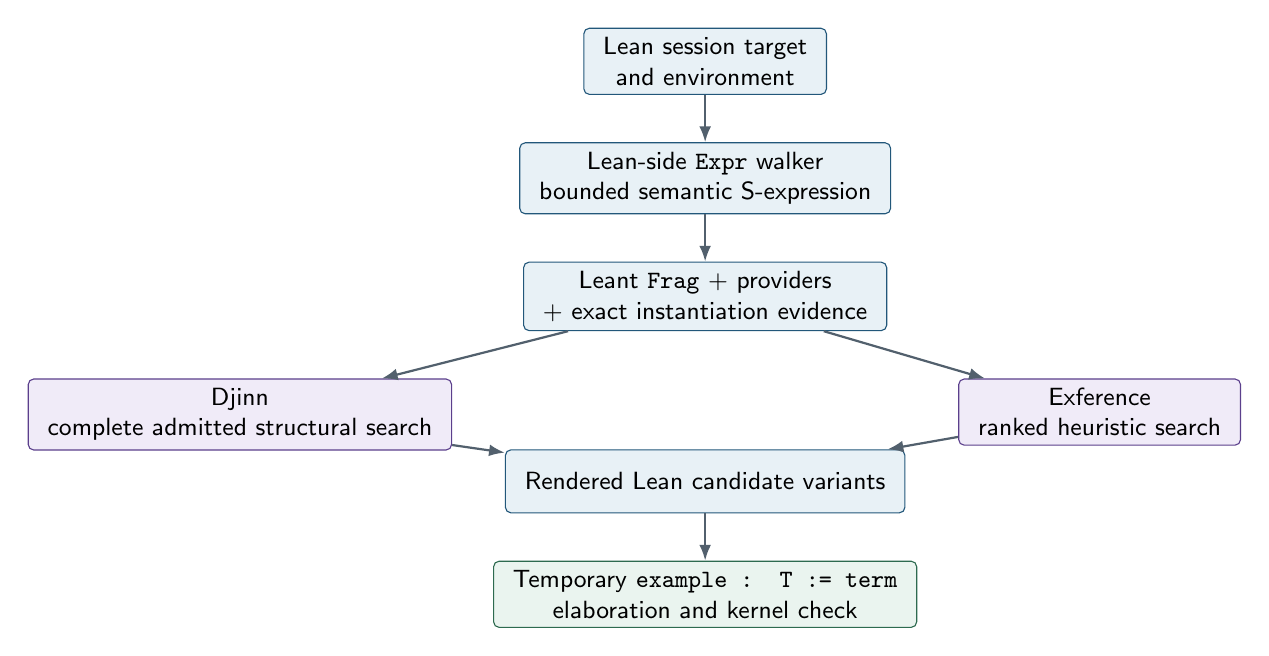
\begin{tikzpicture}[
  node distance=6mm and 9mm,
  every node/.style={font=\small\sffamily},
  box/.style={draw=Accent,rounded corners=2pt,fill=AccentLight,align=center,minimum height=8mm,inner xsep=7pt},
  engine/.style={draw=Purple,rounded corners=2pt,fill=PurpleLight,align=center,minimum height=8mm,inner xsep=7pt},
  check/.style={draw=Green,rounded corners=2pt,fill=GreenLight,align=center,minimum height=8mm,inner xsep=7pt},
  arr/.style={-{Latex[length=2mm]},thick,color=Slate}
]
\node[box] (lean) {Lean session target\\and environment};
\node[box,below=of lean] (sexp) {Lean-side \code{Expr} walker\\bounded semantic S-expression};
\node[box,below=of sexp] (frag) {Leant \code{Frag} + providers\\+ exact instantiation evidence};
\node[engine,below left=of frag] (djinn) {Djinn\\complete admitted structural search};
\node[engine,below right=of frag] (exf) {Exference\\ranked heuristic search};
\node[box,below=15mm of frag] (render) {Rendered Lean candidate variants};
\node[check,below=of render] (verify) {Temporary \code{example : T := term}\\elaboration and kernel check};
\draw[arr] (lean) -- (sexp);
\draw[arr] (sexp) -- (frag);
\draw[arr] (frag) -- (djinn);
\draw[arr] (frag) -- (exf);
\draw[arr] (djinn) -- (render);
\draw[arr] (exf) -- (render);
\draw[arr] (render) -- (verify);
\end{tikzpicture}%
}
\end{center}

The final verifier is generated as source text with the essential shape:

\begin{lstlisting}[language=LeanFour,caption={Current Leant acceptance boundary}]
set_option autoImplicit true in
noncomputable example : (goal) := (candidate)
\end{lstlisting}

This is a valuable boundary: search, rendering, provider discovery, and even the
protocol parser may be wrong without making Lean accept an ill-typed term. The same
boundary should remain in the first native tactic, where it can be strengthened by
elaborating directly in the saved tactic state rather than in a reconstructed REPL
command.

\section{The admitted structural fragment}

Leant's Lean-side serializer elaborates the target and walks the resulting \code{Expr}.
The Haskell-side \code{Frag} distinguishes:

\begin{itemize}
  \item arrows, products, sums, top, bottom, and lowered forms of equivalence and
        negation;
  \item explicit and implicit quantification over sorts;
  \item instance-implicit binders that are erased for search but retained as rendering
        slots;
  \item exact, closed contextual class evidence attached to a particular provider
        assignment;
  \item opaque variables and atoms with a safety bit controlling negative claims;
  \item proper-type applications with variable or exact nominal heads;
  \item non-recursive and recursive inductive occurrences, including parameterized
        families and bounded constructor inventories;
  \item an explicit depth-truncation marker.
\end{itemize}

This is not a generic serialization of Lean syntax. It is a semantic projection into
the part of intuitionistic type structure that Djex can exploit, with explicit markers
for where structure was hidden or truncated. That distinction is exactly what future
proof automation needs: projections should carry their loss, not merely a Boolean
``supported'' flag.

\section{Evidence and progress are already separated}

The public synthesis result distinguishes candidate production, refutation, and
bounded failure:

\begin{lstlisting}[language=HaskellLite,caption={Simplified current Leant outcome type}]
data SynthOutcome
  = SynthCandidates [[String]] [String]
  | SynthRefuted Bool
  | SynthNoTerm [String]
\end{lstlisting}

The Boolean on \code{SynthRefuted} records whether the projection was sufficiently
complete and free of unsafe opaque atoms for the negative verdict to be advertised as
sound. Exference never contributes negative evidence merely because its budget ended.
Progress notes distinguish step, choice-point, candidate, queue, and depth limits.

This evidence/progress split should be preserved verbatim in a future shared protocol.
It prevents a common automation bug: conflating ``the search did not find a term'' with
``no term exists.'' Z3 has the analogous three-way result
\code{sat}/\code{unsat}/\code{unknown}; a unified API should not flatten either
system into success/failure.

\section{Current finite bounds are part of the contract}

At the reviewed revision, Leant's live exact-provider discovery deliberately uses
small, testable bounds. Among the important limits are:

\begin{itemize}
  \item at most six leading type binders opened on one provider;
  \item at most 32 active instance heads inspected in resolver order;
  \item at most 16 alpha-distinct assignment vectors retained per provider;
  \item at most 32 provider/vector associations passed into search;
  \item at most six arguments in one exact vector;
  \item a residual first-order kind-arrow bound of 64;
  \item a bounded vector of visible forall-domain tags;
  \item bounded candidate, display, and verification windows;
  \item bounded Exference queue and step policies.
\end{itemize}

The current functional history widened rank-N and provider instantiation from five to
six binders while preserving seven binders as an explicit fail-closed boundary. It
also added canonical higher-kinded \code{Prod} and \code{Sum} assignments at total
arity two while retaining conservative failure for unsupported structural heads and
legacy payloads. These are signs of healthy engineering: bounds are observable,
tested, and associated with evidence strength.

A future native tactic should expose such bounds as structured diagnostics and cache
keys. It should not silently vary them based on thread timing or solver load.

\section{Djinn and Exference form a useful internal portfolio}

Djinn and Exference have complementary semantics:

\begin{itemize}
  \item \Djinn performs a terminating, complete search for its admitted LJT-oriented
        structural fragment. When projection completeness is established, exhaustion
        can support a negative claim about that abstract problem.
  \item \Exference performs ranked heuristic synthesis under explicit budgets. It is
        often better at useful compositions, but exhaustion carries no negative
        meaning.
  \item Combined mode uses a fair bounded merge rather than allowing one engine's
        repeated candidates to crowd the other out.
  \item Live providers are tried in bounded widening stages. Djinn can begin with the
        highest-ranked provider and expand geometrically; Exference retains its own
        rated full-inventory lane.
\end{itemize}

This is already the seed of the larger portfolio proposed in this report. Z3 should be
added as an orthogonal semantic service, not as a replacement for either structural
engine.

\section{Where the current representation blocks deeper cooperation}

The current public candidate is a group of rendered strings. That is sufficient for
final re-elaboration, but it loses information needed by a cooperative tactic:

\begin{itemize}
  \item stable identity of every local hypothesis and provider occurrence;
  \item the expected type at every subexpression;
  \item which type arguments were synthesized and why;
  \item constructor and case-branch source identities;
  \item residual constraints and holes;
  \item sharing between repeated subterms;
  \item provenance and ranking contributions;
  \item the exact projection loss relevant to this candidate;
  \item a place to attach Z3 models, cores, or branch-feasibility evidence.
\end{itemize}

The durable next representation is a typed candidate graph. Rendered Lean source
should remain as an output view, not the semantic interchange format.

\begin{designbox}[title=Most important Leant evolution]
Change the narrow engine boundary from ``fragment in, ranked strings out'' to
``typed goal snapshot in, ranked proof graphs with residual obligations out.'' Keep
the existing string renderer as one consumer and keep Lean re-elaboration as the
mandatory acceptance boundary.
\end{designbox}

\section{A native tactic need not move Djex into Lean}

There is no requirement to rewrite Djex in Lean or bind the Haskell runtime into the
Lean process. A long-lived worker process is arguably the better first architecture:

\begin{itemize}
  \item it isolates crashes, memory growth, and cancellation;
  \item it can retain Djex sessions and provider caches across goals;
  \item it permits independent release and benchmarking;
  \item the protocol can be recorded for deterministic replay;
  \item Lean remains responsible for all trusted state and final checks.
\end{itemize}

The important change is the interface: a native Lean tactic should own the goal
snapshot and user interaction, while Leant becomes a service that consumes a bounded
projection and returns bounded structured candidates.

\chapter{Z3 as a semantic search and diagnostic engine}
\label{ch:z3}

\section{The useful outputs have different logical strengths}

Z3 exposes solver results, models, unsat cores, proof ASTs, optimization, and
fixedpoint answers. These are not interchangeable.

\begin{longtable}{@{}L{0.18\textwidth}L{0.32\textwidth}L{0.39\textwidth}@{}}
\toprule
\textbf{Z3 artifact} & \textbf{Best use in Lean automation} & \textbf{What must happen before it can close a goal} \\
\midrule
\endhead
\code{sat} model & Counterexample search, candidate refutation, concrete test generation, selector assignment. & Decode into the exact projected domain and re-evaluate all tracked assertions; for theorem-level counterexamples, prove or check realization in Lean. \\
Unsat core & Premise minimization, branch explanation, theorem-retrieval feedback, smaller replay problem. & Reconstruct a proof using the selected premises; the core itself proves nothing in Lean. \\
Quantifier instances / solver trace & Suggest explicit theorem applications and E-matching seeds. & Rebuild well-typed Lean terms for every instantiation and prove the resulting instances. \\
Proof AST / inference log & Diagnostic explanation; possible future rule-by-rule replay. & Parse a versioned rule language and check each step independently, or translate to another checked certificate. \\
Optimize model & Choose smallest premise set, cheapest candidate parameters, invariant coefficients, or branch selectors. & Verify the chosen values and all resulting obligations in Lean. \\
Fixedpoint answer / invariant & Propose loop invariants, Horn summaries, ranking relations, or unreachable states. & Materialize a Lean predicate and prove initialization, preservation, and postcondition/decrease obligations. \\
\code{unknown} + reason & Honest boundary information and fallback routing. & Never closes a goal. Any model returned after \code{unknown} is diagnostic only unless separately validated. \\
\bottomrule
\end{longtable}

The C API documents the key caveats. Proof retrieval requires proof generation to
have been enabled and a preceding \code{unsat} result. Unsat cores are not minimized
by default; minimization options cost additional search. Models are supported after
\code{sat}; after \code{unknown}, a returned model is not guaranteed to satisfy the
assertions, especially quantified assertions. A sound integration should encode these
conditions in constructors rather than rely on callers to remember them.

\section{Z3's strongest early roles}

The highest-value roles do not require parsing a full proof object.

\subsection{Validated counterexample generation}

For exact finite or first-order fragments, Z3 can refute a candidate or conjecture
quickly. A useful result contains:

\begin{itemize}
  \item the exact projection version and source map;
  \item assignments for source-level variables, not raw solver symbols;
  \item the values of tracked intermediate expressions;
  \item a validation record showing that every asserted formula evaluates to true and
        the negated goal evaluates to true in the decoded model;
  \item a warning when the model uses uninterpreted elements that cannot be rendered as
        concrete Lean data.
\end{itemize}

For bit vectors, finite enums, bounded naturals, tuples, and finite algebraic
datatypes, model realization can be exact. For arbitrary functions, infinite types,
quotients, or axiomatized structures, the result may be only an abstract first-order
model. The UI must say which kind it is.

\subsection{Assumption-based unsat cores}

Every candidate premise can be guarded by a Boolean assumption literal:

\begin{lstlisting}[language=SMTLIB,caption={Schematic tracked-premise encoding}]
(declare-const use_h0 Bool)
(declare-const use_h1 Bool)
(assert (=> use_h0 H0))
(assert (=> use_h1 H1))
(check-sat-assuming (use_h0 use_h1 goal_negated))
(get-unsat-core)
\end{lstlisting}

The resulting core can reduce the theorem set handed to \code{grind}, Leant, or a
reconstruction tactic. It can also explain why a candidate branch is impossible. The
core is not necessarily minimum and may vary with solver configuration, so the
integration should distinguish \emph{core}, \emph{locally minimized core}, and
\emph{proven minimal core} if the latter is ever computed.

\subsection{Semantic branch pruning}

A partial proof or program skeleton may introduce Boolean selectors, constructor
choices, arithmetic parameters, or finite branch conditions. Z3 can check whether the
current accumulated constraints are satisfiable before Leant expands the branch. This
is especially useful for Exference-like search, but it must be an effectful outer
scheduler rather than an \code{unsafePerformIO} call hidden inside a pure search
function.

\subsection{Template solving and optimization}

Linear invariant templates, ranking functions, finite lookup tables, branch guards,
and arithmetic witnesses can be represented by unknown coefficients. Z3 can solve or
optimize those coefficients. Lean then receives concrete terms and proves the
resulting verification conditions. This is a cleaner use of SMT than trying to
translate an entire dependent proof.

\section{Proof logging is useful but not yet the trust boundary}

The pinned Z3 tree includes an example of inference logging, replay, and optional
self-validation for a SAT+EUF-oriented configuration. The example explicitly notes
that some quantifier instantiations can be syntactically checked while others are
validated by another SMT call. This is valuable engineering support, but it is not an
independent proof checker in Lean. The same implementation family is helping validate
its own trace, and supported inference kinds depend on solver configuration.

A future proof-object project should therefore be scoped by theory and strategy. For
example:

\begin{enumerate}
  \item use Z3 only to select premises and instances;
  \item reconstruct EUF equalities with Lean congruence lemmas;
  \item dispatch arithmetic leaves to Lean arithmetic tactics;
  \item dispatch propositional leaves to a checked SAT certificate;
  \item leave unsupported rules as explicit residual goals;
  \item record the original proof object for diagnostics but do not make it trusted.
\end{enumerate}

This resembles the current \repo{lean-smt} strategy with cvc5: translate a goal, replay
what is supported, and expose proof holes as ordinary Lean goals. That precedent shows
that partial replay is useful; it also argues against waiting for universal coverage.

\section{Recent Z3 history reinforces the fail-closed design}

Recent changes around quantifier elimination, higher-order matching, polymorphic TPTP
translation, model-based projection, cross-platform determinism, and optimization
soundness demonstrate both Z3's strength and the difficulty of treating a fast solver
as a monolithic oracle. Several fixes explicitly downgrade unsupported dependent or
polymorphic shapes to a ``gave up'' result rather than returning a potentially
unsound theorem. Other changes address solver-path instability caused by hashes or C++
argument evaluation order.

The lesson is not that Z3 is unreliable; mature solvers improve precisely by finding
and fixing such cases. The lesson is that Lean integration should be revision-pinned,
strategy-pinned where reproducibility matters, explicit about \code{unknown}, and
constructed so that a solver defect cannot create a kernel theorem without passing an
independent check.

\section{Candidate theory frontier}

A pragmatic first theory frontier is:

\begin{longtable}{@{}L{0.18\textwidth}L{0.28\textwidth}L{0.36\textwidth}L{0.10\textwidth}@{}}
\toprule
\textbf{Theory} & \textbf{Early Z3 role} & \textbf{Lean proof path} & \textbf{Phase} \\
\midrule
\endhead
Propositional / EUF & Cores, instances, congruence plans, branch pruning. & \code{grind}, simplifier, explicit congruence/equality proof. & 1 \\
Linear integer arithmetic & Models, infeasibility, coefficients, premise cores. & \code{omega}, \code{lia}, or \code{grind} arithmetic extension. & 1 \\
Bit vectors & Counterexamples, branch pruning, arithmetic simplification hints. & \code{bv_decide} and checked LRAT. & 1 \\
Finite datatypes & Concrete models, constructor choices, disjointness/injectivity facts. & Cases, constructor theorems, \code{grind}. & 1 \\
Arrays & Counterexamples and select/store lemma plans. & Rewriting plus extensionality; residual goals allowed. & 2 \\
Linear real/rational arithmetic & Models, cores, coefficients. & Lean linear arithmetic, depending on imports. & 2 \\
Quantified first-order logic & Instance suggestions and premise selection. & Explicit theorem applications + \code{grind}; no raw \code{unsat} trust. & 2 \\
Horn/fixedpoint & Candidate invariants and summaries. & VC generation and checked induction. & 3 \\
Nonlinear arithmetic & Counterexamples, bounded templates, occasional proof plans. & \code{grobner}, normalization, or residual goals; Z3 may return \code{unknown}. & 3 \\
Strings, sequences, regex, floating point & Diagnostics and domain-specific experiments. & Requires dedicated reflection/reconstruction libraries. & \priodefer \\
\bottomrule
\end{longtable}

\chapter{Trust model and result-strength lattice}
\label{ch:trust}

\section{The trusted computing base}

The minimal trusted base should remain:

\begin{itemize}
  \item the Lean kernel and the declarations imported by the user's environment;
  \item the elaborator and metaprograms used to construct the final proof term;
  \item any small certificate checker whose correctness theorem is used;
  \item the projection correctness lemmas needed by that checker.
\end{itemize}

Leant, Djex, Z3, the worker protocol, search heuristics, model printers, premise rankers,
and proof renderers should be untrusted. They may cause failure, delay, or poor
suggestions, but not an invalid theorem.

There is an additional policy question: Lean permits axioms and unsafe computation in
the surrounding environment. A kernel-checked term may depend on axioms. The tactic
should therefore distinguish \emph{kernel accepted} from \emph{axiom-free under a
chosen environment policy}. Optional post-checks analogous to \code{#print axioms}
can report dependencies, but they are separate from solver integration.

\section{A result lattice, not a Boolean}

A common protocol should use constructors with monotone logical strength. One possible
ordering is:

\begin{enumerate}
  \item \textbf{ProofAccepted}: a Lean term has been elaborated at the exact target and
        kernel-checked.
  \item \textbf{CertificateAccepted}: a Lean checker accepted a certificate and its
        soundness theorem produced the target proof.
  \item \textbf{ProofReconstructed}: external evidence was replayed into a Lean proof;
        after checking, this normally becomes \textbf{ProofAccepted}.
  \item \textbf{SkeletonAccepted}: a Lean \code{refine} term was accepted but leaves
        typed residual goals.
  \item \textbf{CounterexampleValidated}: a model was decoded and independently
        re-evaluated in an exact reflected fragment.
  \item \textbf{AbstractModel}: a first-order model satisfies the projection but is not
        known to realize concrete Lean values.
  \item \textbf{UnsatCoreHint}: a subset of translated assumptions used by the solver.
  \item \textbf{NoCandidateWithinBounds}: a finite search frontier ended without a
        candidate.
  \item \textbf{AbstractRefutation}: a complete abstract calculus refuted the projected
        sequent, together with a projection-adequacy label.
  \item \textbf{Unknown}: timeout, resource limit, unsupported theory, incomplete
        quantifier search, interruption, or protocol failure.
\end{enumerate}

Only the first two constructors close a goal directly. The third is an intermediate
implementation state that should be immediately checked. The fourth intentionally
changes the proof state. The remainder are diagnostics or search guidance.

\section{Formal direction of projection guarantees}

Let a Lean proof state be written informally as
\(\Gamma \vdash T\), and let \(P\) project it to an external problem.

For \emph{positive proof search}, no global theorem about \(P\) is required if every
returned candidate \(t\) is elaborated against the original target:

\[
\operatorname{elab}_{\Gamma}(t) : T
\quad\Longrightarrow\quad
\Gamma \vdash t : T.
\]

Projection bugs merely lose candidates or waste time.

For an external \emph{unsatisfiability} result to prove the Lean goal without replay,
one needs a soundness/adequacy bridge of the form

\[
\text{Lean counterexample to }(\Gamma \vdash T)
\quad\Longrightarrow\quad
\text{model of }P(\Gamma \land \neg T).
\]

Then external unsatisfiability rules out every Lean counterexample admitted by the
stated scope. Establishing such a theorem for general dependent type theory is much
harder than checking a proposed term. This is why proof reconstruction should be the
default.

For an external \emph{sat model} to be a concrete Lean counterexample, the required
direction is different: the model must decode to actual Lean values and evaluation
must commute with the projection. This can be proved for reflected finite domains,
bit vectors, and selected first-order datatypes; it should not be assumed for opaque
uninterpreted sorts.

\section{Projection reports}

Every projected query should carry a structured report, for example:

\begin{lstlisting}[language=LeanFour,caption={Schematic projection report}]
structure ProjectionReport where
  exactConnectives       : Array SourceId
  opaqueAtoms            : Array SourceId
  erasedTypeclassBinders : Array SourceId
  monomorphizedDecls     : Array Name
  approximations         : Array Approximation
  depthTruncations       : Array SourceId
  unsupportedTerms       : Array UnsupportedTerm
  modelRealization       : ModelRealizationLevel
  negativeAdequacy       : NegativeAdequacyLevel
\end{lstlisting}

A single \code{Bool} named \code{complete} is not enough once multiple solvers and
subgoals are involved. One approximation may be harmless for positive term
re-elaboration but fatal for a countermodel or abstract refutation.

\section{Protocol and parser trust}

Even when external outputs are untrusted, protocol parsers must be hardened because
they run inside or adjacent to the theorem prover process. The protocol should have:

\begin{itemize}
  \item an explicit schema version and capability negotiation;
  \item exact Lean, Leant, Djex, and solver revision identifiers;
  \item bounded node counts, nesting depth, string length, integer width, and vector
        length;
  \item no executable Lean source embedded in semantic metadata;
  \item stable numeric IDs rather than relying on pretty-printed names;
  \item a cryptographic or collision-resistant hash of the goal snapshot;
  \item rejection of stale results when the goal or environment revision changes;
  \item explicit \code{unknown}, cancellation, timeout, and partial-result messages;
  \item deterministic replay logs suitable for regression tests.
\end{itemize}

Leant's current bounded S-expression parser and fail-closed exact-provider metadata are
a good precedent. The proposed typed protocol should preserve that discipline.


\chapter{Unified proof-automation architecture}
\label{ch:architecture}

\section{Overview}

The proposed system has five layers, shown in \cref{fig:unified-architecture}.

\begin{figure}[H]
\centering
\resizebox{\textwidth}{!}{%
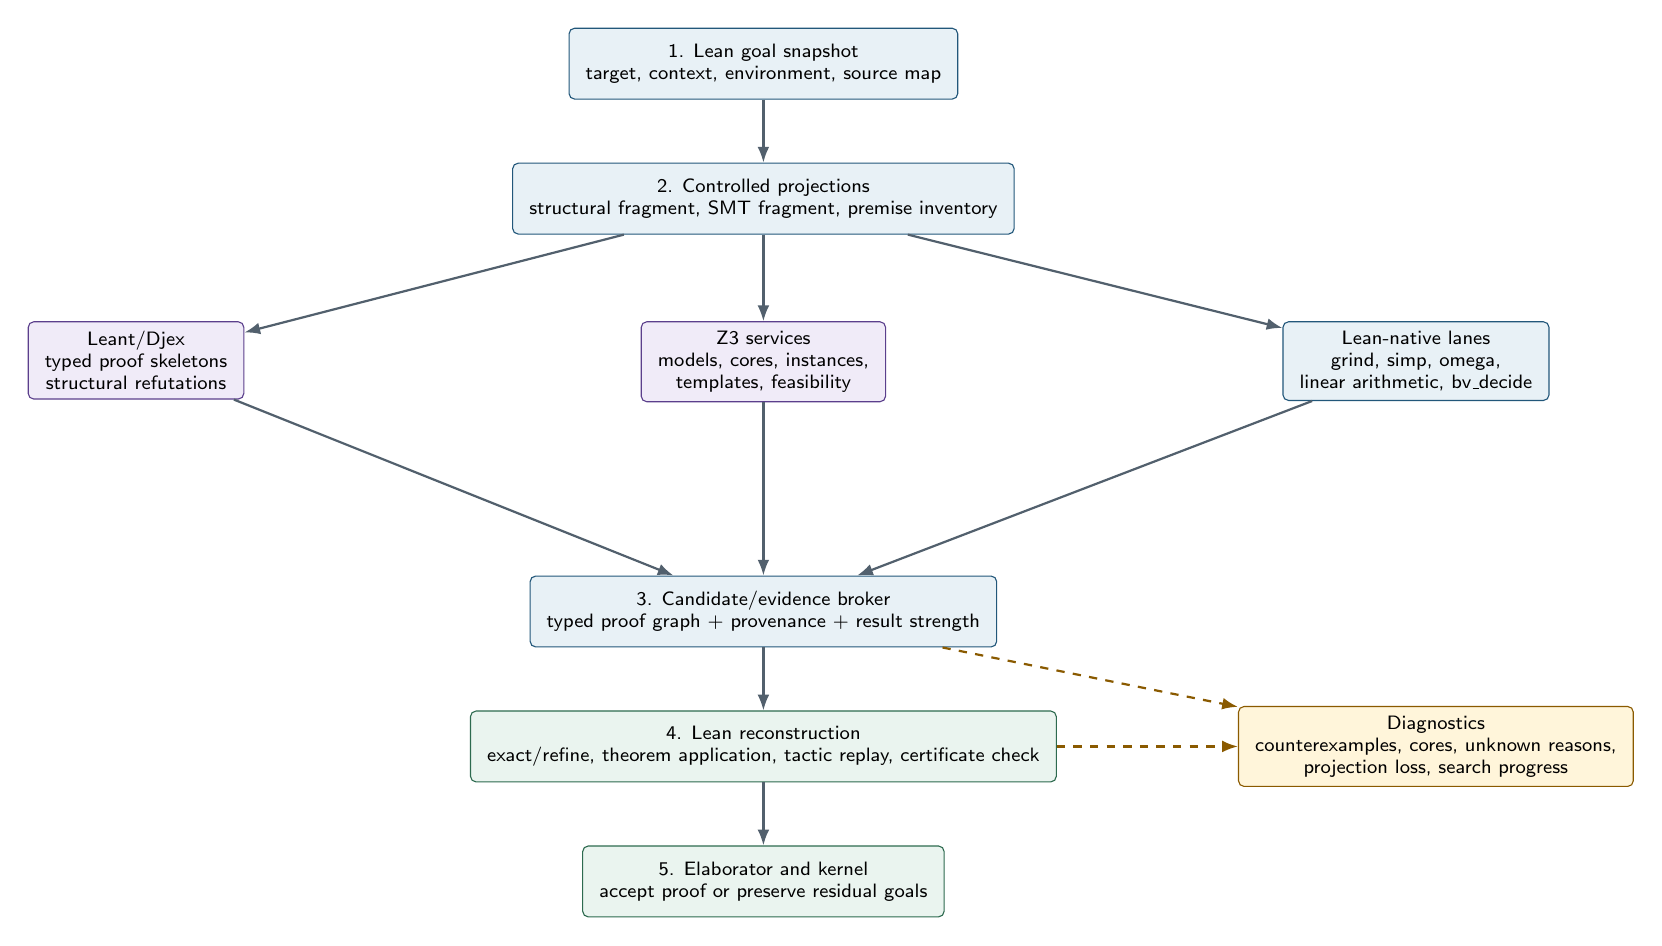
\begin{tikzpicture}[
  node distance=8mm and 10mm,
  every node/.style={font=\scriptsize\sffamily},
  leanbox/.style={draw=Accent,rounded corners=2pt,fill=AccentLight,align=center,minimum height=9mm,inner xsep=6pt},
  extbox/.style={draw=Purple,rounded corners=2pt,fill=PurpleLight,align=center,minimum height=9mm,inner xsep=6pt},
  checkbox/.style={draw=Green,rounded corners=2pt,fill=GreenLight,align=center,minimum height=9mm,inner xsep=6pt},
  diagbox/.style={draw=Gold,rounded corners=2pt,fill=GoldLight,align=center,minimum height=9mm,inner xsep=6pt},
  arr/.style={-{Latex[length=2mm]},thick,color=Slate},
  darr/.style={-{Latex[length=2mm]},thick,dashed,color=Gold}
]
\node[leanbox] (state) {1. Lean goal snapshot\\target, context, environment, source map};
\node[leanbox,below=of state] (project) {2. Controlled projections\\structural fragment, SMT fragment, premise inventory};
\node[extbox,below left=11mm and 34mm of project] (leant) {Leant/Djex\\typed proof skeletons\\structural refutations};
\node[extbox,below=11mm of project] (z3) {Z3 services\\models, cores, instances,\\templates, feasibility};
\node[leanbox,below right=11mm and 34mm of project] (native) {Lean-native lanes\\grind, simp, omega,\\linear arithmetic, bv\_decide};
\node[leanbox,below=22mm of z3] (broker) {3. Candidate/evidence broker\\typed proof graph + provenance + result strength};
\node[checkbox,below=of broker] (recon) {4. Lean reconstruction\\exact/refine, theorem application, tactic replay, certificate check};
\node[checkbox,below=of recon] (kernel) {5. Elaborator and kernel\\accept proof or preserve residual goals};
\node[diagbox,right=23mm of recon] (diag) {Diagnostics\\counterexamples, cores, unknown reasons,\\projection loss, search progress};
\draw[arr] (state) -- (project);
\draw[arr] (project) -- (leant);
\draw[arr] (project) -- (z3);
\draw[arr] (project) -- (native);
\draw[arr] (leant) -- (broker);
\draw[arr] (z3) -- (broker);
\draw[arr] (native) -- (broker);
\draw[arr] (broker) -- (recon);
\draw[arr] (recon) -- (kernel);
\draw[darr] (broker) -- (diag);
\draw[darr] (recon) -- (diag);
\end{tikzpicture}%
}
\caption{Recommended architecture. External engines never mutate the proof state
directly; they return typed artifacts to a Lean-owned broker and reconstruction layer.}
\label{fig:unified-architecture}
\end{figure}

The key object is not an SMT formula or a rendered term. It is a \emph{goal snapshot}
with several projections and a \emph{typed proof graph} whose holes can be delegated to
different solvers.

\section{Goal snapshots}

A snapshot must contain enough information to reject stale or ill-scoped results while
remaining serializable. One schematic Lean-side representation is:

\begin{lstlisting}[language=LeanFour,caption={Schematic Lean-owned goal snapshot}]
structure GoalSnapshot where
  snapshotId       : UInt64
  target           : Expr
  localContext     : LocalContext
  localInstances   : LocalInstances
  levelParams      : Array Name
  metavariableCtx  : MetavarContext
  transparency     : TransparencyMode
  environmentHash  : ByteArray
  sourceMap        : SourceMap
  options          : Options
  dependencySlice  : Array Name
\end{lstlisting}

Not all fields should cross the process boundary. The worker receives a projection
whose nodes refer to stable \code{SourceId}s. The full \code{Expr}, local context, and
metavariable context remain in Lean and are used during reconstruction.

A dependency slice is preferable to hashing the entire environment. It can include the
declarations referenced by the target, local hypothesis types, selected premises, and
provider signatures. This gives meaningful cache invalidation without requiring a
complete module hash. For strict reproducibility, the replay log should also record
the Lean executable revision and imported module fingerprints.

\section{A common candidate and evidence broker}

Each lane should return an artifact with common metadata:

\begin{lstlisting}[language=LeanFour,caption={Schematic common external result}]
structure ExternalCandidate where
  snapshotId  : UInt64
  candidateId : UInt64
  payload     : CandidatePayload
  provenance  : Provenance
  projection  : ProjectionReport
  evidence    : ExternalEvidence
  ranking     : RankingData
  progress    : ProgressReport
\end{lstlisting}

\code{CandidatePayload} may contain a proof graph, a set of derived facts, a theorem
instantiation plan, a model, a premise core, or an invariant template. The broker does
not infer logical strength from the producer name; the producer must supply an
evidence constructor that the Lean side validates structurally.

The broker is also where duplicates are removed. Deduplication should use normalized
semantic nodes and source identities before display limits are applied. Leant already
deduplicates candidate spellings before bounded scheduling; the shared broker should
generalize this to proof graphs and derived facts.

\section{Typed proof graphs}

A graph rather than a tree permits sharing of repeated subproofs and common residual
obligations. A simplified node vocabulary is:

\begin{lstlisting}[language=LeanFour,caption={Schematic proof-graph vocabulary}]
inductive ProofNode
  | exact       (term : TermRef)
  | intro       (binder : BinderRef) (body : NodeId)
  | apply       (function : TermRef) (arguments : Array NodeId)
  | constructor (ctor : Name) (fields : Array NodeId)
  | cases       (scrutinee : FVarRef) (branches : Array CaseBranch)
  | have        (type : TypeRef) (proof body : NodeId)
  | rewrite     (rule : TheoremRef) (direction : Bool) (body : NodeId)
  | induction   (major : FVarRef) (motive : TypeRef)
                (branches : Array CaseBranch)
  | tactic      (capability : Capability) (inputFacts : Array FactRef)
  | hole        (holeId : HoleId) (expected : TypeRef)
                (context : ContextSlice) (capabilities : CapabilitySet)

structure ProofGraph where
  nodes     : Array ProofNode
  root      : NodeId
  sharing   : Array SharingConstraint
  sourceMap : SourceMap
\end{lstlisting}

The graph uses stable references, not embedded pretty-printed Lean expressions. A
\code{TermRef} may designate a local hypothesis, global declaration, literal,
constructor, or a small source-independent term AST. During reconstruction, Lean
resolves every reference in the saved context and checks every expected type.

\section{Residual obligations are a feature}

Traditional external tactics are often all-or-nothing: either the solver closes the
goal or it reports failure. Typed holes make partial automation compositional. A
Leant skeleton may solve the higher-order shape while delegating an arithmetic leaf to
\code{omega}; Z3 may identify two required instances while leaving an array
extensionality lemma to \code{grind}; an induction planner may construct the recursor
while leaving the invariant step as a user-visible goal.

A reconstruction result can therefore be:

\begin{lstlisting}[language=LeanFour,caption={Schematic reconstruction result}]
inductive ReconstructionResult
  | closed   (proof : Expr) (audit : AuditTrail)
  | refined  (proof : Expr) (goals : Array MVarId) (audit : AuditTrail)
  | rejected (reason : ReconstructionError) (audit : AuditTrail)
\end{lstlisting}

This representation aligns naturally with \code{TryThis}: a closed result becomes an
\code{exact} suggestion; a refined result becomes a \code{refine} suggestion whose
remaining goals are checked in the restored tactic state.

\section{Capability-directed hole routing}

Each hole should have a cheap syntactic and semantic capability analysis:

\begin{itemize}
  \item propositional/EUF;
  \item linear integer arithmetic;
  \item linear ordered-ring arithmetic;
  \item polynomial identity;
  \item bit-vector decision problem;
  \item finite datatype case split;
  \item array select/store;
  \item structural term synthesis;
  \item induction or recursion required;
  \item theorem retrieval required;
  \item unsupported/dependent.
\end{itemize}

The scheduler can then route a hole to a small set of plausible lanes instead of
running every engine. Capability analysis must be conservative: ``unknown'' means the
hole may still be attempted by generic Lean tactics, not that it is unprovable.

\section{Proof plans and diagnostics share source identities}

The same \code{SourceId} should identify a local hypothesis in:

\begin{itemize}
  \item the structural Leant fragment;
  \item the SMT declaration and tracked assertion;
  \item a library-suggestion item;
  \item a \code{grind} theorem or fact;
  \item an unsat core;
  \item a proof-graph application node;
  \item the final user-visible source range.
\end{itemize}

This avoids fragile name matching. It also lets the UI say, for example, ``Z3 used
hypotheses \code{h1}, \code{h4}, and \code{h7}; Leant's candidate uses \code{h1} and
\code{h4}; \code{grind} closed the remaining arithmetic goal using \code{h7}.''

\chapter{A native Leant tactic}
\label{ch:native-leant}

\section{Why this is the highest-leverage first step}

Leant's current REPL proves that the core search and verification path works, but a
separate session has unavoidable friction:

\begin{itemize}
  \item the user must restate or replay the exact context;
  \item source locations and editor actions are indirect;
  \item the final candidate is checked in a temporary command rather than the exact
        saved tactic state;
  \item residual goals cannot be returned naturally;
  \item cooperation with \code{grind}, local tactics, and premise selectors is
        awkward;
  \item cancellation and stale-result handling are not integrated with the editor.
\end{itemize}

A native tactic removes all of these without changing the synthesis algorithms.

\section{Proposed commands}

The initial package can expose four commands:

\begin{description}[style=nextline,leftmargin=1.8em]
  \item[\code{leant?}] Search and show one or more validated pasteable suggestions. It
        never changes the proof state unless the editor action is accepted.
  \item[\code{leant}] Apply the highest-ranked candidate that verifies in the current
        state. If the candidate is a skeleton, leave residual goals.
  \item[\code{leant (engine := djinn|exference|both)}] Select the structural engine and
        expose bounded search options.
  \item[\code{leant_trace}] Produce a diagnostic report containing projection loss,
        provider inventory, candidate rejection reasons, and search progress without
        modifying the goal.
\end{description}

A later \code{solve?} command can include Leant as one lane, but Leant should first be
independently usable and testable.

\section{First implementation: preserve the existing textual boundary}

The minimum viable tactic can deliberately avoid a new proof-graph protocol:

\begin{enumerate}
  \item Snapshot the active \code{MVarId}, target, local context, options, and source
        location.
  \item Use Lean metaprogramming to emit the same bounded semantic fragment that the
        REPL serializer currently emits.
  \item Send the fragment, provider inventory, and exact revision metadata to a
        long-lived \code{leant-server} process.
  \item Receive bounded candidate strings and structured progress data.
  \item Restore the saved tactic state and elaborate each candidate against the exact
        target with no \code{sorry} and normal kernel checking enabled.
  \item Convert accepted candidates into \code{TryThis} suggestions.
  \item Reject the entire response if the snapshot ID or environment fingerprint is
        stale.
\end{enumerate}

This approach reuses the existing acceptance argument. It also supplies an immediate
regression oracle for the later structured protocol: both paths should accept the same
candidate set on the existing transcript suite.

\section{Second implementation: return structured candidates}

The next protocol revision should return a typed proof graph. The Lean side then
constructs an \code{Expr} directly or builds a syntax term only at the final suggestion
stage. Direct expression construction has several advantages:

\begin{itemize}
  \item no accidental name capture or pretty-printer dependence;
  \item exact local declaration identities;
  \item explicit type argument and universe handling;
  \item natural creation of metavariable holes;
  \item better source-level explanation of rejected nodes;
  \item graph sharing and common subproofs;
  \item stable comparison of semantic candidates across engines.
\end{itemize}

The renderer remains important: users need readable source and replayable scripts.
But rendering becomes Lean's responsibility after the graph has already reconstructed
successfully.

\section{Worker protocol}

A line-delimited JSON or length-prefixed binary protocol is suitable. JSON is easier to
record and inspect initially; a compact binary encoding can follow if profiling shows
it matters. A request might have the following conceptual form:

\begin{lstlisting}[language=JSONLite,caption={Illustrative Leant worker request}]
{
  "schema": 1,
  "snapshot": "9f38...",
  "leanRevision": "1d2dde6d64cb...",
  "leantRevision": "0160237e4bdf...",
  "djexRevision": "f50b5eac8672...",
  "goal": { "sort": "prop", "fragment": { ... } },
  "providers": [ ... ],
  "premises": [ ... ],
  "engine": "both",
  "limits": {
    "candidateWindow": 60,
    "verificationWindow": 24,
    "exferenceSteps": 128
  }
}
\end{lstlisting}

Every response should repeat the snapshot ID and include a monotonically increasing
response sequence. Streaming candidates is useful: Lean can verify the first few
while the worker continues searching, then cancel when a satisfactory proof is found.
A candidate message should not imply final search exhaustion; a separate terminal
progress message should report completion or truncation.

\section{Provider and premise selection}

The native tactic can improve Leant's current provider path in two stages.

\subsection{Ranked seed inventory}

Ask \code{LibrarySuggestions} for theorem and definition candidates using a caller
name such as \code{"leant"}. Preserve exact source names and provider-local instance
metadata. Run Leant's established geometric widening over the ranked prefix.

\subsection{Demand-driven expansion}

If a candidate skeleton contains a hole headed by a nominal type or relation, query
for additional providers whose result type or theorem conclusion shares that head.
This avoids serializing a large environment before any structural search occurs.

The provider identity rules in current Leant should remain strict. Exact instance
assignments are attached to the provider that exposed them; another provider with an
alpha-identical type may not borrow the evidence.

\section{Verification in the exact tactic state}

The REPL's temporary \code{example} is strong, but a native tactic can be stronger and
more precise:

\begin{itemize}
  \item elaborate under the saved local context and metavariable context;
  \item require the elaborated type to be definitionally equal to the target;
  \item preserve the user's transparency and option settings where semantically
        appropriate;
  \item reject unresolved synthetic opaque metavariables except intentional skeleton
        holes;
  \item restore the original state after a rejected candidate;
  \item invoke the ordinary kernel type checker; never enable
        \code{debug.skipKernelTC};
  \item record imported axioms and unsafe declarations separately for audit output.
\end{itemize}

Candidate verification should run under a bounded heartbeat and allocation budget so
an adversarial or accidentally enormous term cannot freeze the editor.

\section{Compatibility strategy}

Leant's current live transcripts are verified against Lean 4.31, while the reviewed
Lean head is later development code. The native package should therefore separate:

\begin{itemize}
  \item a thin version-specific Lean projection/reconstruction module;
  \item a versioned, mostly stable semantic protocol;
  \item the independent Haskell search worker;
  \item golden protocol fixtures that can be replayed without starting Haskell;
  \item an integration matrix over supported Lean releases and development heads.
\end{itemize}

This localizes API drift in \code{Expr}, elaborator, module, and tactic internals.

\chapter{Typed, hole-bearing proof synthesis}
\label{ch:skeletons}

\section{From complete terms to proof skeletons}

A complete Leant candidate may fail because one small leaf lies outside the structural
fragment. Typical examples include:

\begin{itemize}
  \item a numeric inequality needed after applying the correct hypothesis;
  \item a field equality after choosing the correct constructor and cases;
  \item a definitional simplification involving a recursive function;
  \item a typeclass or coercion fact that Lean can synthesize but Djex intentionally
        erases;
  \item an array or finite-map lemma;
  \item an induction branch whose propositional shape is easy but whose invariant is
        semantic.
\end{itemize}

An all-or-nothing synthesizer discards the useful structural work. A skeleton should
instead preserve the decisions it can justify and insert typed holes at unsupported
leaves.

\section{Hole creation rules}

A hole should be created only at a boundary that Lean can independently check. Good
boundaries include:

\begin{itemize}
  \item the premise of an application whose function and result type are known;
  \item a constructor field;
  \item a case branch result;
  \item the proof of a local \code{have};
  \item an equality or proposition after normalization;
  \item an induction motive or branch obligation;
  \item a typeclass obligation left to ordinary synthesis.
\end{itemize}

A hole should record its expected type, local context slice, source path, and the
structural choices that depend on it. It should not merely be an untyped placeholder in
a string.

\section{Skeleton search objectives}

Once holes are admitted, candidate ranking must account for them. A useful
lexicographic objective is:

\[
\begin{aligned}
(&\text{unreconstructable holes},\ \text{hole count},\quad
  \text{aggregate hole complexity}, \\
 &\text{external solver cost},\ \text{proof graph size},\quad
  \text{provider penalty}).
\end{aligned}
\]

A complete but enormous term may rank below a short skeleton with one trivial
arithmetic hole. Conversely, a skeleton with an opaque dependent hole should rank
below a complete structural proof.

Hole complexity can combine:

\begin{itemize}
  \item target AST size;
  \item quantifier alternation and universe dependence;
  \item theory classification;
  \item number of relevant hypotheses;
  \item presence of recursive definitions;
  \item expected solver availability;
  \item historical reconstruction success for similar goals.
\end{itemize}

These features affect ranking only; they never affect soundness.

\section{Cooperative completion}

The broker can attempt holes in dependency order:

\begin{enumerate}
  \item run cheap definitional reduction and simplification;
  \item invoke typeclass synthesis for instance holes;
  \item run a matching native decision procedure for exact fragments;
  \item ask Z3 for a counterexample/core/instance plan if semantic guidance is useful;
  \item ask \code{grind} with the reduced premise set;
  \item ask Leant recursively for a structural subproof if the hole exposes new
        structure;
  \item stop at a user-visible residual goal if no checked lane succeeds.
\end{enumerate}

The order should be configurable but deterministic. Each successful hole proof is a
normal Lean expression and can be cached independently.

\section{Shared subgoals and DAG search}

Case analysis and theorem application often generate repeated obligations. A proof
graph can hash normalized hole targets together with the relevant local context slice.
Equivalent holes share one solver task and one proof node. This is particularly useful
for:

\begin{itemize}
  \item symmetric constructor branches;
  \item repeated arithmetic side conditions;
  \item quantified theorem applications at the same type arguments;
  \item induction branches with identical invariant facts;
  \item proof repair after a declaration rename.
\end{itemize}

Context equivalence must be conservative. Alpha-renamed local declarations can be
canonicalized, but extra hypotheses may change typeclass search, reducibility, or
simp behavior. The cache key should include the selected dependency slice rather than
only the target text.

\section{Example: structure first, arithmetic second}

Consider a schematic theorem whose useful proof is ``apply the only function that can
produce the result, build its product argument, then prove a numeric bound.'' Leant can
produce:

\begin{lstlisting}[language=LeanFour,caption={Illustrative reconstructed skeleton}]
by
  intro f h x
  refine f x ?_
  -- goal: index x < bound
\end{lstlisting}

The hole classifier recognizes linear natural-number arithmetic. The broker first
tries \code{omega}; if that fails, it may ask Z3 for a model or premise core, then retry
\code{omega} or \code{grind} with the selected facts. The final proof contains no
reference to Z3 or Leant unless the user chooses to keep the high-level tactic call.

\section{Example: semantic branch pruning}

Suppose Exference considers two constructors whose fields induce arithmetic
constraints. The search graph can emit a partial branch formula for each constructor.
Z3 proves one formula unsatisfiable under the current assumptions. This does not close
the Lean goal, but it can prune that synthesis branch because the final candidate from
that branch would necessarily fail the separately checked side conditions.

To remain safe under projection loss, branch pruning should use one of two policies:

\begin{enumerate}
  \item \textbf{Exact policy}: prune only when the branch formula is an exact
        reflection of the side conditions and the unsat result is reconstructed or
        checked.
  \item \textbf{Heuristic policy}: lower the branch priority but do not delete it. If
        the projection was incomplete or the solver result cannot be checked, search
        may still revisit the branch.
\end{enumerate}

The second policy allows aggressive experimentation without sacrificing completeness
claims of the structural engine.

\section{Skeleton replay and proof readability}

A proof graph should support at least three renderings:

\begin{itemize}
  \item a compact term, suitable for \code{exact};
  \item a tactic-style \code{intro}/\code{refine}/\code{cases} script with named
        residual goals;
  \item an audit view showing provenance, solver calls, core premises, and projection
        loss.
\end{itemize}

The shortest term is not always the best maintained proof. The ranking layer should
permit a ``readable'' mode that prefers named intermediate facts, stable theorem
applications, and native tactics over enormous proof terms.

\chapter{Z3 services for proof writing}
\label{ch:z3-services}

\section{One solver, several narrowly specified services}

The integration should not expose a single operation named \code{solveWithZ3}. It
should expose services with distinct contracts:

\begin{enumerate}
  \item \code{findCounterexample};
  \item \code{findUnsatCore};
  \item \code{proposeInstances};
  \item \code{solveTemplate};
  \item \code{checkBranchFeasible};
  \item \code{proposeInvariant};
  \item \code{obtainProofTrace} for diagnostics or experimental replay.
\end{enumerate}

Each service uses a theory-specific projection, result type, validator, and resource
policy.

\section{A typed SMT query object}

A query should be built from a typed internal SMT AST, not concatenated text. SMT-LIB
may remain the process transport, but the builder should know sorts and source
identities:

\begin{lstlisting}[language=LeanFour,caption={Schematic SMT query object}]
structure SmtQuery where
  logic        : SmtLogic
  declarations : Array SmtDecl
  assertions   : Array TrackedAssertion
  assumptions  : Array AssumptionLiteral
  sourceMap    : SmtSourceMap
  timeoutMs    : Nat
  rlimit       : Option Nat
  randomSeed   : UInt32
  requestModel : Bool
  requestCore  : Bool
  requestProof : Bool
  strategy     : SolverStrategy
\end{lstlisting}

The query builder should reject ill-sorted terms before starting the process. The
serialized script should set every non-default solver option explicitly when
reproducibility matters.

\section{Counterexample service}

\subsection{Exact reflected fragments}

The first counterexample checker should support types with straightforward finite or
computable semantics:

\begin{itemize}
  \item \code{Bool}, finite enumerations, and finite products/sums;
  \item fixed-width \code{BitVec};
  \item bounded \code{Fin n};
  \item integers and naturals where all operations have an exact encoding and returned
        numerals fit the decoder;
  \item non-recursive algebraic datatypes and bounded recursive values;
  \item arrays over finite domains when decoded extensionally or as finite stores.
\end{itemize}

For each supported operator, the reflection layer needs an evaluation theorem or a
trusted computation path checked by Lean. The service can then return a concrete
assignment and a theorem or decidable check showing that the hypotheses hold and the
goal does not.

\subsection{Abstract models}

For uninterpreted sorts and functions, Z3 may return a finite abstract universe and
function tables. This is still useful: it often exposes a missing hypothesis or false
algebraic intuition. The result should be labeled \code{AbstractModel}, rendered with
stable element names, and should not be described as a concrete Lean counterexample
unless a realization bridge exists.

\subsection{Model validation}

Validation should happen independently of the pretty printer:

\begin{enumerate}
  \item parse the model into a typed model AST;
  \item verify that every declaration has the expected sort and arity;
  \item evaluate all ground tracked assertions with a separate evaluator;
  \item for quantifier-free finite domains, enumerate quantified binders if bounded;
  \item reject the model if any required value is absent or outside the supported
        decoder;
  \item only then map values back to source-level terms.
\end{enumerate}

This catches protocol errors and many solver-configuration mistakes. It does not
replace a proof of the reflection semantics, but it makes the result robust.

\section{Unsat-core service}

The core service has three modes:

\begin{description}[style=nextline,leftmargin=1.8em]
  \item[Fast core] Return the solver's assumption core with no minimization.
  \item[Deletion-minimized core] Iteratively remove assumptions and recheck. This is
        deterministic under a fixed order and often produces much smaller replay
        problems.
  \item[Weighted core] Use selectors and optimization or bounded search to prefer
        stable/local/user-specified premises. This need not find a globally minimum
        core to be useful.
\end{description}

A core can guide:

\begin{itemize}
  \item which hypotheses are passed to \code{grind};
  \item which library theorems are retained in a Leant provider stage;
  \item which facts are shown in a human-readable explanation;
  \item which proof dependencies are recorded in a repaired proof;
  \item which assumptions are likely redundant in the theorem statement.
\end{itemize}

The reconstruction layer should always be allowed to use fewer or more premises than
the core. The core is a search hint, not a dependency certificate.

\section{Quantifier-instantiation service}

Z3's E-matching and model-based quantifier mechanisms can discover useful ground
instances. The integration should export them as a plan:

\begin{lstlisting}[language=LeanFour,caption={Schematic theorem instantiation plan}]
structure InstantiationPlan where
  theorem      : TheoremRef
  typeArgs     : Array TermRef
  explicitArgs : Array TermRef
  triggerTerms : Array SmtTermId
  origin       : InstantiationOrigin
  dependencies : Array FactRef
\end{lstlisting}

Lean reconstructs the actual theorem application using its own elaborator. It checks
universe levels, implicit arguments, coercions, typeclass synthesis, and definitional
equality. If the instance is valid, the resulting proposition can be added to
\code{grind} or the local context. If reconstruction fails, the plan is discarded and
the failure reason is recorded.

This service is particularly complementary to Leant. Leant can decide where a
higher-rank hypothesis must be applied; Z3 can suggest the ground arguments that make
its first-order consequence useful.

\section{Template-solving service}

A template consists of a Lean-owned syntax with unknown coefficients or finite
choices. Examples include:

\begin{itemize}
  \item \(a_0 + a_1 x_1 + \cdots + a_n x_n \ge 0\) as a linear invariant;
  \item a lexicographic ranking tuple;
  \item a polynomial equality witness;
  \item a finite decision tree over predicates;
  \item a branch selector for a finite set of lemmas;
  \item a bounded lookup table or finite function;
  \item numeric parameters in a constructive witness.
\end{itemize}

The service returns concrete coefficients and an objective value. It does not return a
proof. Lean substitutes the values into the template and generates the exact proof
obligations. Optimize can minimize coefficient magnitude, number of nonzero terms,
number of selected premises, or a weighted syntactic cost.

\section{Branch-feasibility service}

Partial proof graphs can accumulate semantic constraints. The branch service should
accept only a monotone conjunction of tracked facts and return:

\begin{itemize}
  \item \code{Feasible} with an optional model;
  \item \code{Infeasible} with a core and a reconstruction status;
  \item \code{Unknown} with a reason and consumed budget.
\end{itemize}

An infeasible result may be used to prune only if the reconstruction status is strong
enough for the search's completeness policy. Otherwise it changes ranking but not the
set of explored branches.

\section{Fixedpoint and invariant service}

Z3's fixedpoint engine can solve Horn clauses and often return inductive invariants or
answers useful for reachability. The integration should not attempt to import the
entire answer formula blindly. Instead:

\begin{enumerate}
  \item Lean generates Horn clauses from a selected recursive/loop specification.
  \item The projection records each relation, state component, and transition source.
  \item Z3 proposes a relation interpretation or invariant formula in a restricted
        template language.
  \item Lean parses that formula into a typed predicate.
  \item Lean proves initialization, preservation, exit/postcondition, and termination
        obligations using native tactics and, recursively, the semantic services.
\end{enumerate}

If the answer uses unsupported constructs, it remains a diagnostic. Template-based
invariant extraction is easier to trust and render than arbitrary solver formulas.

\section{Solver process management}

For the first version, a separate Z3 process speaking SMT-LIB is preferable to a C FFI:

\begin{itemize}
  \item process termination is a reliable cancellation fallback;
  \item memory and CPU limits can be enforced by the operating system;
  \item exact scripts can be recorded and replayed;
  \item solver upgrades do not require rebuilding a Lean native extension;
  \item malformed or crashing solver behavior is isolated.
\end{itemize}

A pool of long-lived workers can still use incremental \code{push}/\code{pop}. Each
worker must have a strict state machine so one cancelled query cannot leak assertions
into the next. Periodic worker replacement avoids unbounded memory retention.


\chapter{Theory-specific proof reconstruction}
\label{ch:reconstruction}

\section{Why reconstruction should be theory-specific}

A generic SMT proof is an interleaving of propositional reasoning, congruence,
rewriting, preprocessing, quantifier instantiation, and theory lemmas. Replaying every
internal rule couples Lean to solver implementation details. A smaller design
classifies the final obligations and reconstructs each theory with the proof machinery
Lean already has.

The external solver is then a \emph{proof-plan generator}. It may identify a useful
set of facts, a contradiction core, an equality path, or concrete coefficients. Lean
constructs the actual proof.

\section{Propositional reasoning and EUF}

For quantifier-free propositional logic with equality and uninterpreted functions, a
reconstruction pipeline can be:

\begin{enumerate}
  \item Normalize source propositions into Lean's \code{grind} representation while
        retaining theorem and source IDs.
  \item Ask Z3 for a core, relevant equalities, and optional ground instances.
  \item Add reconstructed instances as ordinary Lean facts.
  \item Invoke \code{grind} on the reduced fact set.
  \item If \code{grind} fails, reconstruct an explicit congruence path or expose the
        equality subgoal.
\end{enumerate}

An equality explanation can be represented as a small DAG:

\begin{lstlisting}[language=LeanFour,caption={Schematic equality explanation}]
inductive EqReason
  | hypothesis  (fact : FactRef)
  | symmetry    (reason : ReasonId)
  | transitivity (left right : ReasonId)
  | congruence  (function : TermRef) (arguments : Array ReasonId)
  | rewrite     (theorem : TheoremRef) (arguments : Array TermRef)
\end{lstlisting}

Lean checks every edge by theorem application. This format is independent of Z3's
internal proof node names and can also be produced by another EUF engine.

\section{Linear integer arithmetic}

Z3 is excellent at finding a contradictory subset, a model, or useful bounds. Lean's
native arithmetic tactics are the preferred proof path:

\begin{itemize}
  \item \code{omega} for Presburger-style natural and integer arithmetic;
  \item \code{lia} or the linear arithmetic extension of \code{grind}, depending on
        the exact target and imports;
  \item simplification and normalization before arithmetic dispatch.
\end{itemize}

The reconstruction plan should map every SMT arithmetic atom back to its Lean
expression. A Z3 core selects the candidate inequalities; Lean reruns the native tactic
on those facts. If the native tactic succeeds, the proof is independent of the solver
result. If it fails because the projection used an unsupported operation or a different
normal form, the result remains a diagnostic.

For an arithmetic witness, Z3 may return a numeral or coefficient vector. Lean
constructs the witness term and proves the required inequalities. This is often more
useful than importing a contradiction proof.

\section{Linear rational and real arithmetic}

The same pattern applies to ordered rings and fields, with two additional cautions:

\begin{itemize}
  \item Lean and SMT must agree on division, inverses, coercions, and side conditions
        such as nonzero denominators.
  \item The available reconstruction tactic depends on imported libraries. A core
        Lean package should not assume all of mathlib, but an optional mathlib adapter
        can use \code{linarith}, \code{nlinarith}, normalization, and ring tactics.
\end{itemize}

The projection should make coercions explicit and reject mixed arithmetic it cannot
normalize soundly.

\section{Bit vectors}

Bit vectors have the cleanest proof-producing path:

\begin{enumerate}
  \item Reify the Lean bit-vector proposition.
  \item Use \code{grind} facts and Z3 only to simplify, find counterexamples, or select
        relevant hypotheses.
  \item Run \code{bv_decide} on the resulting exact proposition.
  \item Check the LRAT certificate in Lean.
\end{enumerate}

Z3 need not be the SAT solver used by \code{bv_decide}; its role can be purely
semantic and diagnostic. If a future Z3 path emits a compatible CNF certificate, it
can feed the same checker, but that is an optimization rather than a design
requirement.

The recent \code{bv_decide}/\code{grind} integration is a template for sharing facts:
\code{grind} normalizes equalities and theory information, then \code{bv_decide}
encodes the relevant equivalence classes into its reflected problem.

\section{Algebraic datatypes}

For finite and algebraic datatypes, Z3 can suggest constructor equalities,
disjointness, injectivity, and case splits. Lean reconstruction should use the exact
inductive declaration:

\begin{itemize}
  \item constructor applications are rebuilt with universe and parameter arguments;
  \item disequality of distinct constructors is proved by no-confusion or generated
        disjointness theorems;
  \item equality of same-constructor applications is decomposed with injectivity;
  \item exhaustive cases are built with the inductive recursor or \code{cases};
  \item recursive values in a countermodel are decoded only under an explicit depth
        bound or finite-domain argument.
\end{itemize}

Leant already serializes bounded constructor inventories and maps private engine names
back to exact Lean constructors. The new source map should be shared with the SMT
projection to prevent duplicate datatype identity mechanisms.

\section{Arrays, maps, and extensionality}

Arrays are more delicate because SMT arrays are total extensional functions with
\code{select} and \code{store}, while Lean libraries expose several data structures and
possibly different semantics. A safe first adapter should target a specific reflected
array type and theorem set.

Reconstruction may use:

\begin{itemize}
  \item read-over-write lemmas;
  \item simplification of equal and unequal indices;
  \item extensionality to reduce array equality to pointwise equality;
  \item finite-domain enumeration when the index type is finite;
  \item residual pointwise goals when full automation fails.
\end{itemize}

A Z3 model of an array often uses a default value plus finitely many stores. This can
be rendered as an abstract diagnostic even when no exact Lean array term is available.
Concrete counterexamples require an agreed array representation.

\section{Polynomial identities and nonlinear arithmetic}

For pure polynomial equalities, Z3 is not needed for the proof. It may help discover a
normalization or parameter assignment; Lean should close the identity with a ring or
Groebner-style tactic. For inequalities and nonlinear integer arithmetic, Z3 is
incomplete and may return \code{unknown}. The system should use it for models and
bounded templates while retaining ordinary Lean residual goals for unsupported
proofs.

A useful hybrid is:

\begin{enumerate}
  \item Z3 finds candidate coefficients or a counterexample;
  \item Lean substitutes coefficients;
  \item \code{grobner}, normalization, interval facts, or imported mathlib tactics
        discharge algebraic leaves;
  \item any transcendental or genuinely nonlinear reasoning remains explicit.
\end{enumerate}

\section{Quantifiers}

Quantifier reconstruction should never accept ``Z3 instantiated something'' as a
proof step. Each instance must be traced to a source theorem or local hypothesis and
rebuilt in Lean. The main services are:

\begin{itemize}
  \item monomorphization proposals;
  \item ground term discovery;
  \item trigger and instance proposals;
  \item premise cores after instantiation;
  \item finite-domain enumeration where exact.
\end{itemize}

The reconstructed instances can then be consumed by \code{grind}. Unsupported
higher-order or dependent instances are discarded. Leant's rank-N machinery is useful
for deciding the structural placement of applications that an SMT solver sees only
after monomorphization.

\section{A reconstruction registry}

Theory support should be registered by exact reflected operators and result strengths:

\begin{lstlisting}[language=LeanFour,caption={Schematic theory adapter registry}]
structure TheoryAdapter where
  name          : Name
  recognizes    : GoalSnapshot -> MetaM Recognition
  project       : GoalSnapshot -> Recognition -> MetaM SmtQuery
  validateModel : SmtModel -> MetaM ModelValidation
  reconstruct   : UnsatEvidence -> MetaM ReconstructionResult
  capabilities  : CapabilitySet
  version       : Nat
\end{lstlisting}

Adapters compose only through explicit shared terms. A query mixing unsupported
operators is split into holes or rejected rather than silently approximated.

\chapter{Cooperation with \code{grind}, \code{TryThis}, and premise selection}
\label{ch:grind-integration}

\section{Three integration stages}

A sensible progression avoids depending immediately on unstable internals.

\subsection{Stage 1: sibling tactic portfolio}

Each lane receives the same goal snapshot but operates independently:

\begin{itemize}
  \item Leant returns a term or skeleton;
  \item Z3 returns a model/core/instance plan;
  \item Lean-native tactics attempt the goal directly;
  \item the broker reconstructs and ranks validated results.
\end{itemize}

Communication occurs through ordinary Lean facts and residual goals. This stage can be
implemented entirely with public metaprogramming interfaces and \code{TryThis}.

\subsection{Stage 2: fact exchange}

The portfolio shares a normalized fact layer:

\begin{itemize}
  \item \code{grind} preprocessing yields canonical expressions and relevant
        equivalence classes;
  \item Z3 receives only the facts and symbols in the selected dependency slice;
  \item reconstructed Z3 instances or arithmetic facts are inserted back as Lean
        theorems;
  \item Leant receives those facts as additional structural premises;
  \item \code{bv_decide} and other reflected solvers consume the same equalities.
\end{itemize}

This mirrors the current \code{bv_decide} integration without requiring Z3 to become a
native \code{grind} solver.

\subsection{Stage 3: solver extension}

Only after an external extension API stabilizes should a Z3-backed component live
inside \code{GrindM}. Such an extension might receive internalized atoms and equality
updates, maintain an incremental solver, and inject checked conflict lemmas. It must
still reconstruct every injected fact. The benefit is lower serialization overhead
and tighter propagation; the cost is coupling to \code{grind}'s backtracking,
canonicalization, and proof-placeholder discipline.

\section{How Leant can consume \code{grind} facts}

Leant should not serialize the entire E-graph. It needs a selected view:

\begin{itemize}
  \item canonical representatives for local terms used in the target or providers;
  \item proved equalities and disequalities with source proof references;
  \item simplified types and propositions;
  \item constructor facts and no-confusion consequences;
  \item selected arithmetic facts that have ordinary Lean proof expressions.
\end{itemize}

These facts can enter Djex as ordinary provider premises with exact names. A candidate
that uses them is rendered back to the corresponding Lean proof reference. If a fact
was only a transient internal inference with no reconstructed proof, it must not cross
the boundary.

\section{How Z3 can consume \code{grind} facts}

Z3 benefits from the same canonicalization:

\begin{itemize}
  \item fewer duplicate ground terms;
  \item smaller congruence problems;
  \item explicit constructor equalities;
  \item normalized arithmetic expressions;
  \item source-level theorem identities already attached to facts;
  \item better core explanations.
\end{itemize}

The projection should still be built from Lean expressions, not from untyped printed
E-graph nodes. Every exported fact must have a Lean proof or be a source hypothesis.

\section{Premise selection loop}

A useful closed loop is:

\begin{enumerate}
  \item \code{LibrarySuggestions} proposes a ranked premise prefix.
  \item Leant and/or \code{grind} attempt the goal.
  \item Z3 checks the first-order projection and returns a core or model.
  \item Core members receive a temporary score boost; model-visible missing symbols
        trigger a focused retrieval expansion.
  \item Reconstruction attempts the reduced problem.
  \item The final accepted proof records actual theorem dependencies, which can be
        used as offline training or evaluation data.
\end{enumerate}

No online score update should mutate global project state by default. The tactic may
use ephemeral per-goal feedback; persistent learning should be an explicit tool with
versioned data.

\section{Suggestion ranking}

Validated scripts can be ranked by a weighted tuple:

\begin{itemize}
  \item closed proof before skeleton;
  \item fewer residual goals;
  \item fewer imported or nonlocal premises;
  \item smaller proof term or script;
  \item stable named theorems before fragile unfolding;
  \item native checked tactic before a large opaque generated term;
  \item fewer axiomatic dependencies under the chosen policy;
  \item lower measured replay time;
  \item engine-specific relevance score.
\end{itemize}

Ranking occurs after verification. A high-scoring raw candidate that does not
elaborate has no standing.

\section{A proposed \code{solve?} command}

The portfolio command might behave as follows:

\begin{lstlisting}[language=LeanFour,caption={Illustrative portfolio command}]
example (n m : Nat) (h1 : n <= m) (h2 : m < n + 1) : n = m := by
  solve?
-- Candidate lanes:
--   omega: accepted
--   leant + omega skeleton: accepted, larger
--   z3 core -> omega: accepted, same premises h1 h2
-- Try this:
--   omega
\end{lstlisting}

The UI should show one default suggestion and make the audit comparison available on
demand. The shortest accepted native tactic should normally win; Leant and Z3 add
value on goals where native tactics need structural guidance, better premises, or
semantic witnesses.

\chapter{Quantifiers, higher-order structure, and theorem retrieval}
\label{ch:quantifiers}

\section{The structural/semantic division is especially valuable here}

SMT solvers operate most naturally on monomorphic first-order formulas. Lean goals
frequently contain polymorphic declarations, higher-order functions, typeclass
arguments, dependent binders, and proof terms. Leant/Djex is better positioned to
construct the Curry--Howard application structure; Z3 is better positioned to choose
useful ground instances once a safe first-order view exists.

A cooperative path is:

\begin{enumerate}
  \item Leant identifies a hypothesis or provider whose result shape can solve the
        current structural goal.
  \item The proof graph exposes typed argument holes, including type arguments and
        theorem premises.
  \item Lean reifies supported first-order argument constraints.
  \item Z3 proposes ground terms or a small set of instance assignments.
  \item Lean elaborates the exact application and inserts the resulting proposition
        into \code{grind}.
  \item Remaining higher-order or dependent arguments stay as explicit holes.
\end{enumerate}

This avoids erasing higher-order structure merely to make the entire goal look like
SMT-LIB.

\section{Bounded rank-N planning}

Leant's current six-binder boundary is a deliberate finite search contract. Future
work should improve \emph{planning} before merely raising the bound:

\begin{itemize}
  \item infer which quantified hypotheses can affect the result head;
  \item use type-argument unification to eliminate impossible instantiations;
  \item share repeated instantiation sites;
  \item let Z3 rule out inconsistent finite combinations of ground assignments;
  \item allocate the binder budget adaptively to the most relevant hypotheses;
  \item retain explicit truncation reasons when the frontier is incomplete.
\end{itemize}

The structural engine remains responsible for legal application and lambda placement.
Z3 may choose among a finite set of typed assignments but should not invent untyped
polymorphic terms.

\section{Monomorphization as a proof-producing transformation}

A monomorphizer should return more than a first-order formula. It should return:

\begin{itemize}
  \item the source theorem and exact universe/type arguments;
  \item the instantiated Lean proposition;
  \item a proof expression obtained by applying the source theorem;
  \item the first-order encoding of that proposition;
  \item the dependency relation between generated instances;
  \item bounds and truncation status.
\end{itemize}

Then every SMT premise has an ordinary Lean proof before it reaches Z3. The solver can
select or combine instances without adding trust.

The current \repo{lean-smt} use of \repo{lean-auto} for monomorphization is a relevant
comparison. A Z3 integration can reuse or interoperate with such infrastructure rather
than design a second incompatible instance language.

\section{Model-guided instance generation}

When Z3 returns a model for a quantified approximation, the model can suggest which
terms distinguish the current candidate. A bounded loop is:

\begin{enumerate}
  \item solve the current finite instance set;
  \item inspect model values at trigger terms;
  \item generate source-typed candidate instances;
  \item validate and add them in Lean;
  \item repeat under an explicit round and instance budget.
\end{enumerate}

Failure to reach unsatisfiability is \code{Unknown} or
\code{NoInstanceWithinBounds}, never a proof that the theorem is false. A concrete
model can still be shown if it validates the finite approximation.

\section{Theorem retrieval beyond symbol overlap}

Premise selection can combine several signals:

\begin{itemize}
  \item constants and type heads in the target;
  \item Leant provider-result compatibility;
  \item \code{grind} E-matching symbols and pattern availability;
  \item historical theorem dependencies;
  \item Z3 core frequency;
  \item model-visible missing relations;
  \item embeddings of normalized theorem statements;
  \item local declaration proximity and namespace/module preference.
\end{itemize}

The selector should return scored source declarations, not pretranslated SMT axioms.
Lean decides whether and how each theorem is instantiated.

\section{Abduction and missing-lemma suggestions}

A useful proof-writing feature is to ask what additional proposition would make the
current proof go through. General logical abduction is hard, but bounded forms are
practical:

\begin{itemize}
  \item choose a subset of candidate library lemmas using Boolean selectors;
  \item solve for a linear inequality template;
  \item infer an equality between existing terms;
  \item select a constructor invariant from a finite vocabulary;
  \item propose a missing precondition from a bounded atom set.
\end{itemize}

The result should be presented as a conjectured helper lemma or missing assumption.
Lean must prove it separately. This can turn a failed automated proof into a useful
next editing action rather than a generic timeout.

\chapter{Induction, recursion, invariants, and termination}
\label{ch:induction}

\section{Why induction is the next major frontier}

Most current structural and SMT automation is strongest on local, nonrecursive goals.
Real Lean developments frequently fail at choosing:

\begin{itemize}
  \item the induction variable or recursor;
  \item a generalized motive;
  \item which variables must be reverted;
  \item an auxiliary invariant;
  \item a termination measure;
  \item a strengthening of the statement that is stable under recursion.
\end{itemize}

These choices are not well served by one engine. Leant can synthesize recursor and
constructor structure; Z3 can solve semantic templates and find counterexamples to
weak invariants; Lean can generate and check the exact induction obligations.

\section{Induction-skeleton synthesis}

Extend the proof graph with an induction node that records:

\begin{itemize}
  \item the major premise or recursive argument;
  \item the exact recursor or induction theorem;
  \item the proposed motive;
  \item generalized local variables;
  \item branch contexts and induction hypotheses;
  \item residual branch goals;
  \item termination or well-foundedness obligations where applicable.
\end{itemize}

Leant can search a bounded set of structurally plausible induction plans. Plans are
reconstructed immediately in Lean; ill-typed motives or recursor applications are
rejected before semantic solving.

\section{Invariant synthesis loop}

For a loop, recursive function, state machine, or inductive proof, use a template-
checking loop:

\begin{enumerate}
  \item Lean chooses the exact state variables and generates verification conditions:
        initialization, preservation, exit/postcondition, and optionally decrease.
  \item A bounded template language is built from source terms and relations.
  \item Z3 finds coefficients or selectors satisfying a finite encoding of the VCs, or
        returns a countermodel to the current template.
  \item The candidate invariant is reconstructed as a Lean predicate.
  \item Lean attempts all VCs with native tactics and the proof portfolio.
  \item A failed VC yields a checked counterexample or a stronger template request.
  \item The process terminates under explicit rounds, coefficient bounds, and template
        growth limits.
\end{enumerate}

The final theorem depends only on the Lean-checked invariant proof. Z3 is a generator.

\section{Linear and lexicographic ranking functions}

Termination measures are well suited to SMT template solving. For a transition
\(x \to x'\), search for coefficients \(a_i\) such that

\[
\rho(x)=a_0+\sum_i a_i x_i,
\qquad
\rho(x)\ge 0,
\qquad
\rho(x') < \rho(x).
\]

For lexicographic tuples, add selector variables identifying the first decreasing
component and prove nonincrease of earlier components. Lean receives the concrete
measure and proves the well-founded decrease obligation. Recent Lean work on
well-founded and state-dependent measures in verification-condition generation makes
this direction particularly compatible with the native ecosystem.

\section{Predicate discovery from cores and models}

A template vocabulary can grow from failed attempts:

\begin{itemize}
  \item unsat cores identify predicates essential to preservation;
  \item models expose state components or relations not constrained by the invariant;
  \item constructor branches contribute discriminator predicates;
  \item array models contribute selected indices;
  \item theorem retrieval contributes named domain lemmas;
  \item Leant contributes structurally available projections and recursive fields.
\end{itemize}

This is a proof-oriented form of counterexample-guided abstraction refinement. Every
new predicate has a source identity and exact Lean type.

\section{Recursive data and fold lemmas}

For recursive inductives, Leant already distinguishes complete and partial constructor
inventories and uses different projections for Djinn and Exference. Future proof
automation can add \emph{family descriptors}:

\begin{itemize}
  \item exact inductive head and parameters;
  \item constructor fields and recursive positions;
  \item available recursors, folds, maps, and eliminators;
  \item algebraic laws and homomorphism lemmas registered for \code{grind};
  \item size or measure functions;
  \item finite-model bounds for counterexample search.
\end{itemize}

A family descriptor lets Leant synthesize a fold/recursor skeleton while Z3 reasons
about an abstract measure or state relation. The exact recursive proof remains in Lean.

\section{Statement strengthening}

When an induction hypothesis is too weak, bounded strengthening can search a grammar of
candidate conjuncts or generalized variables. Z3 can reject candidates with concrete
countermodels to the step condition. Lean verifies the surviving strengthened theorem.

The UI should show the proposed stronger lemma explicitly. Automatic strengthening
must not silently change the theorem being proved; it should insert a local helper or
suggest a new declaration.

\chapter{Counterexample-guided synthesis and proof repair}
\label{ch:cegis}

\section{CEGIS for proof terms and witnesses}

Leant/Djex can generate structural candidate families; Z3 can distinguish them with
models. A bounded counterexample-guided loop is:

\begin{enumerate}
  \item Leant generates a typed candidate or sketch.
  \item Lean elaborates it and extracts supported behavioral obligations.
  \item Z3 searches for a counterexample to those obligations.
  \item A validated counterexample becomes a new test constraint on the search.
  \item Leant/Exference generates the next candidate under accumulated constraints.
  \item When no counterexample is found, Lean still proves the final obligation; the
        absence of a Z3 model is not accepted as the theorem unless reconstructed.
\end{enumerate}

This is useful for constructive witnesses, finite functions, data-structure
transformations, and proof terms with finite semantic choices. The type system and
structural search guarantee that every candidate is well-formed; semantic constraints
focus the enumeration.

\section{Semantic fingerprints and candidate equivalence}

Many structurally different candidates behave identically on the current finite model
set. The broker can assign a semantic fingerprint: the vector of evaluated outputs or
predicates over validated counterexamples. Exference can keep the cheapest candidate
per fingerprint and avoid spending Lean verification budget on equivalent variants.

This is a heuristic quotient only. Two candidates with the same finite fingerprint
are not definitionally or extensionally equal in Lean. The final selected candidate is
proved independently.

\section{Proof repair after source changes}

A broken proof often retains most of its structure. Store an optional proof graph and
audit trail beside generated scripts. On failure after a refactor:

\begin{enumerate}
  \item re-resolve source declarations by stable names and type fingerprints;
  \item reconstruct the unchanged prefix of the graph;
  \item turn failed nodes into typed holes;
  \item use theorem retrieval to find replacement declarations;
  \item ask Z3 for a core or counterexample explaining changed semantic assumptions;
  \item ask Leant to resynthesize only the affected structural region;
  \item render a new validated script and show the dependency changes.
\end{enumerate}

This is more robust than rerunning a monolithic tactic from scratch and more
maintainable than storing an opaque proof term.

\section{Diagnosing false or underspecified lemmas}

When a goal appears unprovable, the portfolio can produce a structured diagnostic:

\begin{itemize}
  \item Leant reports whether the structural fragment is refuted, incomplete, or
        outside bounds;
  \item Z3 reports a validated or abstract model of the first-order projection;
  \item the premise selector reports potentially missing relevant theorems;
  \item an abduction service proposes bounded missing assumptions;
  \item projection reports identify definitions or dependent structure that prevented
        a strong conclusion.
\end{itemize}

This is often more valuable to a proof author than another tactic timeout.

\section{Synthesis under behavioral constraints}

The same architecture can synthesize a term and its proof together. For example, a
candidate function may be required to preserve list length, maintain a finite-state
invariant, or satisfy a postcondition. Leant builds the term skeleton; Z3 filters
semantic choices and proposes invariants; Lean proves the final specification. This
extends proof automation into verified program synthesis without changing the trust
model.

\section{Limits of finite counterexamples}

Finite testing and bounded models are powerful search tools but provide no completeness
for general Lean propositions. The protocol must record:

\begin{itemize}
  \item domain bounds and enumeration strategy;
  \item whether recursive values were depth-bounded;
  \item whether functions were represented extensionally or as uninterpreted symbols;
  \item whether arithmetic was mathematical, bit-vector, or bounded;
  \item which quantifiers were instantiated rather than universally checked.
\end{itemize}

The UI should say ``no counterexample within bounds'' rather than ``proved''.


\chapter{Concrete protocol and API design}
\label{ch:protocol}

\section{Design goals}

The protocol must support independent evolution of Lean, Leant/Djex, and Z3 while
making semantic drift obvious. Its goals are:

\begin{itemize}
  \item no dependence on pretty-printed Lean syntax for identity;
  \item explicit types, binders, universes, and source references;
  \item bounded parsing and memory use;
  \item streaming candidates and progress;
  \item versioned capabilities;
  \item deterministic recording and replay;
  \item forward-compatible unknown fields;
  \item strong rejection of malformed, stale, or inconsistent data;
  \item separation of semantic payload from user-facing rendering.
\end{itemize}

\section{Stable identities}

The Lean side assigns compact IDs within one snapshot:

\begin{lstlisting}[language=LeanFour,caption={Schematic identity types}]
structure SnapshotId where value : UInt64
structure SourceId   where value : UInt32
structure BinderId   where value : UInt32
structure TermId     where value : UInt32
structure TypeId     where value : UInt32
structure FactId     where value : UInt32
structure NodeId     where value : UInt32
structure HoleId     where value : UInt32
\end{lstlisting}

IDs are never reused within a snapshot. A response carrying an unknown ID is rejected.
A global declaration additionally carries its fully qualified \code{Name}, universe
arity, and a type fingerprint. The fingerprint protects against resolving the same
name to a changed declaration after recompilation.

\section{Semantic term and type AST}

The interchange AST should be smaller than Lean's full \code{Expr} but richer than
Leant's current rendered atoms. It may include:

\begin{itemize}
  \item sorts and universe parameters represented symbolically;
  \item local and global references;
  \item applications with explicit argument visibility;
  \item nondependent and dependent function types;
  \item lambdas and lets where needed for proof graphs;
  \item products, sums, propositions, equality, and selected inductive applications;
  \item literals for supported arithmetic and bit-vector domains;
  \item opaque nodes with exact source IDs and inferred types;
  \item no arbitrary embedded tactic syntax.
\end{itemize}

Every node has a type ID. The parser checks graph acyclicity where required, index
bounds, arities, and sort consistency. Lean nevertheless rechecks the reconstructed
expression; protocol type checking is a robustness and diagnostic feature, not the
final trust boundary.

\section{Binder visibility and implicit information}

Lean elaboration depends on binder information. The protocol must distinguish:

\begin{itemize}
  \item explicit, implicit, strict implicit, and instance-implicit binders;
  \item term binders from type/sort binders;
  \item source-visible names from anonymous/internal names;
  \item binders that Leant erases semantically but must recreate in a lambda;
  \item exact provider type arguments inferred from instance heads;
  \item whether an argument should be emitted explicitly or left for elaboration.
\end{itemize}

Current Leant already records explicit forall visibility, rendering slots for instance
binders, exact provider binder names, kind arities, and semantic forall-domain tags.
The typed protocol should generalize those successful mechanisms rather than replace
them with raw source strings.

\section{Projection capabilities}

The request includes a capability declaration. For example:

\begin{lstlisting}[language=JSONLite,caption={Illustrative capability negotiation}]
{
  "capabilities": {
    "proofGraph": 2,
    "residualHoles": true,
    "rankNBinders": 6,
    "exactProviderAssignments": true,
    "structuralProdSumKinds": true,
    "smt": ["QF_UF", "QF_LIA", "QF_BV", "QF_AUFBV"],
    "modelValidation": ["finite", "bitvector", "integer"],
    "evidence": ["candidate", "core", "model", "instancePlan"]
  }
}
\end{lstlisting}

A worker must not infer permission from a schema version. Unsupported requested
capabilities produce a structured refusal before search starts.

\section{Progress and truncation}

Progress is a first-class stream:

\begin{lstlisting}[language=LeanFour,caption={Schematic progress report}]
inductive TruncationReason
  | timeout
  | heartbeatLimit
  | memoryLimit
  | candidateLimit
  | choicePointLimit
  | queuePruned (count : Nat)
  | binderLimit (observed supported : Nat)
  | providerLimit
  | instanceLimit
  | depthLimit
  | solverUnknown (reason : String)
  | interrupted

structure ProgressReport where
  phase       : Name
  explored    : Nat
  candidates  : Nat
  elapsedMs   : Nat
  truncation  : Array TruncationReason
  completeFor : Array Capability
\end{lstlisting}

The phrase \code{completeFor} is important. A search may be complete for the pure
structural core while incomplete for provider widening or quantifier instantiation.

\section{Evidence payloads}

A common evidence type can be:

\begin{lstlisting}[language=LeanFour,caption={Schematic evidence vocabulary}]
inductive ExternalEvidence
  | candidateOnly
  | structuralDerivation (derivation : DerivationGraph)
  | structuralRefutation (refutation : RefutationGraph)
                         (adequacy : NegativeAdequacyLevel)
  | model (model : SmtModel) (validation : ModelValidationLevel)
  | unsatCore (facts : Array FactId) (minimality : CoreMinimality)
  | instantiations (plans : Array InstantiationPlan)
  | theoryPlan (plan : TheoryProofPlan)
  | certificate (format : CertificateFormat) (bytes : ByteArray)
  | proofTrace (format : ProofTraceFormat) (bytes : ByteArray)
  | invariantTemplate (template : TemplateAssignment)
  | noEvidence
\end{lstlisting}

Only \code{certificate} in a registered checked format and a successfully reconstructed
proof can become goal-closing evidence. \code{proofTrace} is deliberately weaker.

\section{Candidate rejection taxonomy}

Rejected candidates should be classified rather than silently skipped:

\begin{itemize}
  \item stale snapshot;
  \item unknown or changed declaration;
  \item malformed graph or out-of-range ID;
  \item type mismatch at a node;
  \item unresolved universe constraint;
  \item failed typeclass synthesis;
  \item unsupported coercion or elaboration ambiguity;
  \item unresolved non-hole metavariable;
  \item kernel rejection;
  \item timeout or allocation limit during verification;
  \item residual hole outside the advertised capability;
  \item forbidden axiom/unsafe dependency under policy;
  \item duplicate of an earlier semantic candidate.
\end{itemize}

These categories are invaluable for improving the renderer and protocol. A raw
``candidate failed'' message hides whether the search or the bridge is responsible.

\section{Schematic Lean reconstruction API}

\begin{lstlisting}[language=LeanFour,caption={Possible Lean-side API surface}]
namespace ProofPortfolio

structure ReconstructConfig where
  allowResidualGoals : Bool := true
  maxResidualGoals   : Nat := 8
  verifyKernel       : Bool := true
  axiomPolicy        : AxiomPolicy := .report

opaque snapshotGoal : MVarId -> MetaM GoalSnapshot
opaque projectForLeant : GoalSnapshot -> MetaM LeantRequest
opaque projectForSmt   : GoalSnapshot -> TheoryAdapter -> MetaM SmtQuery

opaque reconstructGraph :
  GoalSnapshot -> ProofGraph -> ReconstructConfig -> MetaM ReconstructionResult

opaque validateModel :
  GoalSnapshot -> SmtQuery -> SmtModel -> MetaM ModelValidation

opaque replayTheoryPlan :
  GoalSnapshot -> TheoryProofPlan -> MetaM ReconstructionResult

opaque addTryThisSuggestion :
  GoalSnapshot -> ReconstructionResult -> TacticM Unit

end ProofPortfolio
\end{lstlisting}

The opaque declarations above indicate module boundaries, not axioms in the final
implementation.

\section{Schematic Haskell worker API}

\begin{lstlisting}[language=HaskellLite,caption={Possible Leant/Djex worker boundary}]
data SearchRequest = SearchRequest
  { requestSnapshot   :: SnapshotId
  , requestGoal       :: TypedFragment
  , requestProviders  :: [Provider]
  , requestPremises   :: [Premise]
  , requestCapabilities :: CapabilitySet
  , requestLimits     :: SearchLimits
  }

data SearchEvent
  = CandidateEvent CandidateGraph Provenance RankingData
  | DiagnosticEvent Diagnostic
  | ProgressEvent ProgressReport
  | FinishedEvent Completion

runSearch :: SearchRequest -> ConduitT () SearchEvent IO ()
\end{lstlisting}

Internally, pure Djinn and Exference search can remain pure. The outer driver handles
streaming, timeouts, semantic callbacks, and cancellation.

\chapter{Scheduling, caching, and process isolation}
\label{ch:scheduling}

\section{A deterministic portfolio scheduler}

Parallelism is useful, but proof automation must remain reproducible enough to debug.
The scheduler should define a deterministic priority and budget policy even when lanes
run concurrently.

A reasonable default sequence is:

\begin{enumerate}
  \item cheap simplification, assumption, constructor, and native exact tactics;
  \item capability-specific native solver;
  \item Leant Djinn small structural search;
  \item premise selection and \code{grind};
  \item Leant combined structural search;
  \item Z3 counterexample/core/instance service;
  \item reconstruction with reduced premises;
  \item larger Exference or invariant/template search;
  \item return the best validated result available under the total budget.
\end{enumerate}

Lanes may overlap in wall-clock execution, but candidate ranking and tie-breaking use
stable lane priorities, semantic cost, and candidate IDs. A faster nondeterministic
arrival should not permanently change the default proof script when two accepted
results are equivalent in cost.

\section{Cancellation}

Cancellation must propagate through:

\begin{itemize}
  \item editor/tactic interruption;
  \item Lean meta computation;
  \item Leant worker request;
  \item pure search forcing;
  \item Z3 process or API interrupt;
  \item candidate verification;
  \item pending cache writes.
\end{itemize}

Every request has a cancellation token and deadline. A cancelled worker is not reused
unless its protocol state is known to be clean. If a Z3 incremental session cannot be
safely unwound after interruption, terminate and replace the process.

\section{Cache layers}

Useful caches include:

\begin{description}[style=nextline,leftmargin=1.8em]
  \item[Projection cache] Normalized structural and SMT projections keyed by the goal
        snapshot and adapter version.
  \item[Provider cache] Leant's existing environment/session replay cache, keyed by
        import history and exact provider query.
  \item[Candidate cache] Proof graphs from Leant/Djex keyed by typed fragment,
        provider inventory, limits, and engine revision.
  \item[Solver cache] Z3 model/core/template results keyed by canonical SMT query,
        solver revision, strategy, and options.
  \item[Hole-proof cache] Kernel-accepted proofs for normalized residual goals under a
        conservative context dependency slice.
  \item[Rendering cache] Validated source scripts keyed by proof graph and pretty-
        printer/options version.
\end{description}

A cache hit never bypasses verification. Cached proof graphs are reconstructed against
the current snapshot; cached scripts are re-elaborated; cached models are revalidated
if used as current diagnostics.

\section{Incremental sessions}

Leant already has a pure replay plan distinguishing reuse, suffix replay, and full
replay when the interactive command history changes. The native service should expose
this mechanism explicitly. Similarly, a Z3 session can retain stable declarations and
use \code{push}/\code{pop} for goal-specific assertions.

Incrementality must not leak semantic context:

\begin{itemize}
  \item every declaration belongs to an environment generation;
  \item every goal runs at a known solver stack depth;
  \item cancellation restores or destroys the session;
  \item proof/model/core options are fixed per worker class;
  \item random seeds and tactics are recorded;
  \item assertions are named with snapshot-scoped IDs.
\end{itemize}

\section{Resource isolation}

External workers should run with:

\begin{itemize}
  \item memory and CPU limits;
  \item bounded stdout/stderr capture;
  \item no network access by default;
  \item a controlled working directory;
  \item explicit executable paths and hashes;
  \item no ability to modify source files;
  \item sanitized environment variables;
  \item process replacement after protocol errors or excessive memory growth.
\end{itemize}

This is ordinary robustness, not an implication that the tools are malicious. Search
engines routinely encounter pathological inputs.

\section{Deterministic replay bundles}

Every nontrivial failure should be exportable as a small replay bundle containing:

\begin{itemize}
  \item the semantic request with source text redacted optionally;
  \item exact executable revisions and options;
  \item provider/premise inventory fingerprints;
  \item worker and solver event stream;
  \item candidate graph or proof trace;
  \item reconstruction error and Lean messages;
  \item random seeds and resource limits.
\end{itemize}

Replay bundles make cross-platform solver differences and version regressions
tractable. They also permit protocol fuzzing without a live Lean project.

\chapter{User experience and proof presentation}
\label{ch:ux}

\section{Commands and their promises}

A coherent command family should make result strength visible:

\begin{longtable}{@{}L{0.18\textwidth}L{0.38\textwidth}L{0.34\textwidth}@{}}
\toprule
\textbf{Command} & \textbf{Behavior} & \textbf{Promise} \\
\midrule
\endhead
\code{leant?} & Show validated structural term or skeleton suggestions. & Every shown closed term elaborates at the current goal; skeletons list residual goals. \\
\code{leant} & Apply the best validated Leant result. & Changes proof state only through accepted Lean expressions. \\
\code{z3?} & Show a reconstructed proof suggestion, core, or model depending on capability. & Output labels distinguish proof, concrete counterexample, abstract model, core, and unknown. \\
\code{counterexample?} & Search exact and bounded model adapters. & Never claims a theorem; reports realization and bounds. \\
\code{solve?} & Run the proof-producing portfolio and show the best validated script. & Only checked proof lanes are offered as goal-closing actions. \\
\code{explain_failure} & Summarize structural bounds, projection loss, models, cores, and rejected candidates. & Diagnostic only. \\
\bottomrule
\end{longtable}

\section{Result wording}

The UI should use exact language. Examples:

\begin{itemize}
  \item ``Proof accepted by Lean.''
  \item ``Proof skeleton accepted; 2 residual goals remain.''
  \item ``Concrete counterexample validated for \code{x = 0}, \code{y = 1}.''
  \item ``Abstract first-order model found; uninterpreted element \code{U!0} has no
        concrete Lean decoder.''
  \item ``Z3 returned an unsat core containing 4 of 19 translated premises; Lean
        reconstruction succeeded using 3 premises.''
  \item ``No Leant candidate found within the six-binder and 60-candidate bounds.''
  \item ``Djinn refuted the exact pure structural projection.''
  \item ``Solver returned unknown: incomplete quantified reasoning.''
\end{itemize}

Phrases such as ``Z3 proved'' should be reserved for a result that was actually
reconstructed or certificate-checked in Lean.

\section{Readable proof selection}

The portfolio should offer modes:

\begin{description}[style=nextline,leftmargin=1.8em]
  \item[Compact] Prefer the shortest accepted term or tactic.
  \item[Readable] Prefer named intermediate facts, explicit cases, and stable theorem
        applications.
  \item[Robust] Prefer proofs with fewer unfolding dependencies, smaller premise sets,
        and successful replay across normalization variants.
  \item[Diagnostic] Preserve solver provenance, cores, and comments in a generated
        proof draft.
\end{description}

The generated source can include comments only in diagnostic mode; the semantic proof
graph remains comment-free.

\section{Interactive steering}

Users should be able to constrain the portfolio without writing a new tactic:

\begin{lstlisting}[language=LeanFour,caption={Illustrative steering options}]
by
  solve? (using := [h1, h2, theoremName])
         (without := [expensiveLemma])
         (engines := [.grind, .leant, .z3])
         (maxPremises := 24)
         (allowInduction := false)
         (counterexamples := .finite 8)
\end{lstlisting}

These options influence search only. The final proof remains ordinary Lean.

\section{Explanations from proof graphs}

A proof graph can generate a concise explanation:

\begin{quote}
Introduce \code{x}. Apply \code{map_preserves} to the local hypothesis \code{h}; this
creates a structural equality and a numeric bound. The equality is solved by
simplification. Z3 selected hypotheses \code{hBound} and \code{hNonneg} as an
unsatisfiable arithmetic core; \code{omega} reconstructed the bound. The resulting
term was accepted by Lean.
\end{quote}

This is more reliable than asking an external solver to narrate an opaque proof trace.
The explanation is generated from checked nodes and source identities.

\section{Proof drafts and helper lemmas}

When a goal is not closed, the tactic can still emit a useful draft:

\begin{lstlisting}[language=LeanFour,caption={Illustrative partial proof draft}]
by
  induction xs with
  | nil => simp
  | cons x xs ih =>
      refine constructor
      . exact ?length_bound
      . simpa using ih
\end{lstlisting}

The editor can focus the first residual hole. A separate action may insert a proposed
helper lemma or invariant statement above the theorem, but this must be explicit
because it changes the source-level proof plan.

\chapter{Implementation roadmap and acceptance gates}
\label{ch:roadmap}

\section{Principle of the roadmap}

Each milestone should end with a useful, independently testable feature. Later stages
must not be prerequisites for trusting earlier ones. In particular, Z3 proof-object
support is not required for a valuable counterexample/core/instance service.

\section{Milestone 0: shared fixtures and revision discipline}

\textbf{Deliverables}

\begin{itemize}
  \item Pin exact Lean, Leant, Djex, and Z3 revisions in integration tests.
  \item Extract current Leant serializer, provider, candidate, and transcript fixtures.
  \item Define snapshot IDs, source IDs, progress, truncation, and result-strength
        constructors.
  \item Build protocol fuzz tests and malformed-input limits.
  \item Establish a benchmark corpus spanning propositional structure, providers,
        rank-N goals, arithmetic leaves, bit vectors, datatypes, and negative cases.
\end{itemize}

\textbf{Acceptance gate}: all existing Leant transcript candidates are replayable from
recorded fixtures; malformed and stale messages fail closed; benchmark results record
exact revisions and limits.

\section{Milestone 1: native \code{leant?} using current candidate strings}

\textbf{Deliverables}

\begin{itemize}
  \item Lean tactic package and long-lived Leant worker.
  \item Goal snapshot, current semantic fragment request, provider query, cancellation,
        and streaming progress.
  \item Candidate verification in the exact saved tactic state.
  \item \code{TryThis} suggestions and a detailed rejection trace.
  \item Compatibility tests over supported Lean versions.
\end{itemize}

\textbf{Acceptance gate}: every displayed candidate elaborates and kernel-checks at the
current goal; editor cancellation leaves no worker/session corruption; existing live
Leant examples work without manually replaying them in a separate REPL.

\section{Milestone 2: typed proof graphs and residual holes}

\textbf{Deliverables}

\begin{itemize}
  \item Versioned semantic term/type AST and stable IDs.
  \item Djex/Leant typed candidate projection.
  \item Lean reconstruction to \code{Expr} and \code{refine} skeletons.
  \item Hole capability analysis and native tactic dispatch.
  \item Graph sharing, semantic deduplication, and readable rendering.
\end{itemize}

\textbf{Acceptance gate}: candidates that formerly failed because of one arithmetic or
simplification leaf now produce accepted skeletons; no embedded worker source text is
required for semantic identity; all holes have Lean-checked expected types.

\section{Milestone 3: Z3 counterexamples and unsat cores}

\textbf{Deliverables}

\begin{itemize}
  \item Typed SMT AST and process pool.
  \item Exact QF\_UF, QF\_LIA, QF\_BV, and selected finite-datatype adapters.
  \item Independent model parser/evaluator and concrete/abstract model labels.
  \item Fast and deletion-minimized assumption cores.
  \item Source mapping and editor diagnostics.
\end{itemize}

\textbf{Acceptance gate}: every reported concrete model is independently re-evaluated;
\code{unknown} is preserved; models after \code{unknown} are never labeled
counterexamples; core-guided premise reduction demonstrably reduces replay problems
without changing trust.

\section{Milestone 4: theory-specific reconstruction}

\textbf{Deliverables}

\begin{itemize}
  \item EUF equality-plan reconstruction.
  \item Core-to-\code{grind} and core-to-arithmetic replay.
  \item Z3-guided \code{omega}/linear arithmetic and \code{bv_decide} dispatch.
  \item Finite datatype constructor/case reconstruction.
  \item Residual-goal fallback for unsupported array and quantified steps.
\end{itemize}

\textbf{Acceptance gate}: a Z3 \code{unsat} closes a goal only after the reconstructed
Lean proof succeeds; disabling Z3 and replaying the generated script still proves the
theorem.

\section{Milestone 5: cooperative \code{solve?} and premise feedback}

\textbf{Deliverables}

\begin{itemize}
  \item Deterministic portfolio scheduler.
  \item Shared normalized fact/source layer with \code{grind}.
  \item \code{LibrarySuggestions} adapter for Leant providers and Z3 feedback.
  \item Candidate ranking modes and proof audit reports.
  \item Cache and replay bundle infrastructure.
\end{itemize}

\textbf{Acceptance gate}: the portfolio never returns a weaker diagnostic when a
checked proof is available; result ordering is stable under repeated runs with fixed
options; shared-state paths outperform independent tactic racing on selected mixed
benchmarks.

\section{Milestone 6: induction and invariant synthesis}

\textbf{Deliverables}

\begin{itemize}
  \item Induction-skeleton proof nodes and bounded motive/generalization search.
  \item Linear and lexicographic invariant/ranking templates.
  \item Z3 template and fixedpoint adapters.
  \item Lean VC generation and recursive portfolio solving.
  \item Explicit helper-lemma/strengthening suggestions.
\end{itemize}

\textbf{Acceptance gate}: every synthesized invariant and termination measure is
materialized as Lean syntax and all VCs are kernel-checked; failed or bounded searches
produce counterexamples/unknown labels rather than false success.

\section{Milestone 7: selective certificate and proof-trace replay}

\textbf{Deliverables}

\begin{itemize}
  \item Identify a stable subset of Z3 proof rules or a translation to a standard
        certificate format.
  \item Implement a bounded parser and small Lean checker for that subset.
  \item Fall back to theory reconstruction or residual holes for unsupported rules.
  \item Differentially test checker results against native reconstruction and solver
        self-validation.
\end{itemize}

\textbf{Acceptance gate}: the checker has an explicit Lean soundness theorem; no
unsupported proof rule is accepted; solver upgrades cannot silently change the rule
semantics.

\section{Recommended stopping points}

Milestones 1 through 4 already form a highly useful system. Milestone 5 adds integrated
polish and performance. Milestone 6 is a research-rich extension. Milestone 7 should be
undertaken only if profiling shows that native reconstruction leaves a significant and
valuable class of goals unsolved.

\chapter{Evaluation methodology}
\label{ch:evaluation}

\section{Metrics}

The evaluation should separate search quality, reconstruction quality, proof quality,
and diagnostics.

\begin{longtable}{@{}L{0.25\textwidth}L{0.65\textwidth}@{}}
\toprule
\textbf{Metric} & \textbf{Meaning} \\
\midrule
\endhead
Kernel acceptance rate & Fraction of generated closed candidates accepted at the exact target. \\
Skeleton utility rate & Fraction of skeletons for which native/Z3-guided lanes close at least one residual goal, and fraction fully closed. \\
Time to first accepted proof & End-to-end latency including projection, external search, reconstruction, and checking. \\
Readable-script rate & Accepted results whose rendered script meets size and stability criteria. \\
Candidate rejection distribution & Bridge defects versus genuine search mismatch: names, universes, instances, type mismatch, kernel rejection, resource limit. \\
Premise reduction & Initial suggestions versus Z3 core versus actual dependencies of the accepted proof. \\
Model validation rate & Raw solver models versus independently validated concrete or abstract models. \\
Unknown/truncation rate & Frequency and reasons, grouped by theory and goal shape. \\
Search work & Djinn choice points, Exference nodes/queue pruning, Z3 conflicts/rlimit, generated instances, candidates verified. \\
Residual-goal complexity & Count and capability class before and after portfolio routing. \\
Replay stability & Success under repeated runs, theorem reordering, alpha-renaming, import changes, and supported Lean/Z3 upgrades. \\
Cache effectiveness & Hit rate, revalidation cost, stale rejection rate, and memory footprint. \\
\bottomrule
\end{longtable}

\section{Benchmark strata}

The corpus should contain:

\begin{enumerate}
  \item pure propositional and Curry--Howard combinator goals;
  \item products, sums, equivalence, negation, and finite inductives;
  \item local and library provider compositions;
  \item explicit/implicit/rank-N binders through and beyond the supported boundary;
  \item exact active-instance provider assignments, including higher-kinded cases;
  \item structural skeletons with one or more arithmetic leaves;
  \item EUF and quantified theorem-instantiation problems;
  \item bit-vector verification goals;
  \item finite datatype and array examples;
  \item false statements with concrete and abstract models;
  \item goals requiring induction, invariants, or strengthened hypotheses;
  \item adversarial malformed protocol inputs and resource bombs;
  \item real proofs from Lean core, Std, and selected external projects, respecting
        licensing and dependency constraints.
\end{enumerate}

\section{Baselines}

Compare against:

\begin{itemize}
  \item \code{simp}, \code{grind}, \code{omega}/arithmetic tactics,
        \code{grobner}, and \code{bv_decide} alone;
  \item current Leant REPL behavior at the pinned functional revision;
  \item Leant native tactic without Z3;
  \item Z3 diagnostic/core service without Leant;
  \item independent tactic racing versus shared facts and cores;
  \item \repo{lean-smt} on its supported cvc5 theories where comparison is meaningful;
  \item explicit human-written proofs for readability and replay stability.
\end{itemize}

The objective is not to beat every specialized tactic. The portfolio should invoke the
specialized tactic when it is already the best answer.

\section{Metamorphic tests}

Automation should preserve behavior under transformations that should not affect the
proof problem:

\begin{itemize}
  \item alpha-renaming local hypotheses and binders;
  \item reordering independent hypotheses;
  \item adding irrelevant hypotheses and declarations;
  \item changing user-facing universe parameter names;
  \item replacing a term by a definitionally equal form;
  \item reassociating products/sums where explicit equivalences are supplied;
  \item changing theorem declaration order while retaining names and types;
  \item replaying with a cold versus warm worker cache;
  \item serializing and reparsing the same protocol request;
  \item varying solver seeds where the result strength should remain the same.
\end{itemize}

Candidate ranking may change under some transformations, but logical labels and final
kernel acceptance must not.

\section{Differential tests}

Useful differential checks include:

\begin{itemize}
  \item Z3 model evaluation versus a separate evaluator and Lean computation;
  \item Z3 core replay versus native tactics on the selected facts;
  \item structured Leant reconstruction versus current rendered-string verification;
  \item \code{grind} with and without Z3-proposed instances;
  \item bit-vector counterexamples versus \code{bv_decide};
  \item proof-graph rendering versus direct \code{Expr} reconstruction;
  \item any future proof-trace checker versus solver self-validation and native
        reconstruction.
\end{itemize}

Disagreement is a test failure or an explicit unsupported case, never silently resolved
in favor of the external solver.

\section{Adversarial protocol tests}

Fuzz and hand-write cases with:

\begin{itemize}
  \item cycles in supposedly acyclic graphs;
  \item invalid node IDs and duplicate IDs;
  \item wrong arities, sorts, and binder counts;
  \item huge integers, strings, arrays, and nesting depth;
  \item malicious source names and Unicode edge cases;
  \item stale snapshot IDs and changed declaration fingerprints;
  \item candidates with unresolved metavariables or hidden \code{sorry};
  \item solver output after cancellation;
  \item incomplete JSON/binary frames;
  \item inconsistent progress/completion claims;
  \item proof certificates exceeding declared limits.
\end{itemize}

The expected outcome is a bounded structured error and an unchanged proof state.

\chapter{Risks, semantic traps, and non-goals}
\label{ch:risks}

\section{Semantic mismatch risks}

\subsection{Natural numbers versus integers}

SMT integer subtraction is total and may be negative; Lean natural subtraction is
truncated. Division and modulus conventions also need exact agreement. Projections
must use side conditions or dedicated operators rather than rely on visual similarity.

\subsection{Partial operations}

Field inversion, array indexing wrappers, head/tail operations, and user definitions
may have defaults or require hypotheses. A translator must include the source semantics
and side conditions or leave the term opaque.

\subsection{\code{Prop} versus \code{Bool}}

Lean propositions and Boolean computations are related by reflection lemmas, not
identical. Every conversion must be explicit and reconstructed.

\subsection{Functions and extensionality}

SMT functions and arrays are extensional. Lean function equality requires function
extensionality, available as a theorem/axiom in the environment. The proof audit should
report such dependencies. Models of higher-order functions are generally abstract.

\subsection{Datatypes and recursion}

Z3 algebraic datatypes have first-order semantics; Lean inductives may be indexed,
dependent, nested, quotient-based, or involve proof fields. Only exact admitted
families should be translated structurally. Recursive countermodels need finite
realization or explicit bounds.

\subsection{Type classes and coercions}

Typeclass synthesis can choose evidence based on the current environment and local
instances. Leant's exact provider-assignment discipline should be retained. Z3 should
never model class dictionaries as interchangeable opaque values when their identity
affects elaboration or computation.

\subsection{Definitional equality and transparency}

An SMT projection sees explicit equations; Lean also has definitional reduction under
configurable transparency. Projection and reconstruction should normalize through a
named, recorded policy. A proof that depends on aggressive unfolding may be fragile
and should rank below a stable theorem-based proof when possible.

\subsection{Quotients, proof irrelevance, and subsingletons}

These features can invalidate naive first-order encodings. Treat them as opaque until a
dedicated adapter provides exact theorems.

\section{Engineering risks}

\begin{longtable}{@{}L{0.22\textwidth}L{0.37\textwidth}L{0.31\textwidth}@{}}
\toprule
\textbf{Risk} & \textbf{Failure mode} & \textbf{Mitigation} \\
\midrule
\endhead
Lean API drift & Projection/reconstruction package breaks across releases. & Thin version adapter, protocol fixtures, support matrix, avoid private \code{grind} internals initially. \\
Solver drift & Different models, cores, traces, performance, or proof rules. & Pin revisions/options, record scripts, validate results independently, replace workers cleanly. \\
Search explosion & Combined structural, premise, instance, and semantic search becomes unusable. & Capability routing, explicit budgets, staged widening, core reduction, DAG sharing, deterministic truncation. \\
Poor proof readability & Accepted terms are enormous or fragile. & Post-verification ranking, proof-graph rendering modes, native tactic preference, helper lemmas. \\
Protocol complexity & Bridge becomes harder to maintain than the engines. & Small semantic AST, capability negotiation, generated codecs, bounded schema, replay fixtures. \\
False confidence from models & Abstract/bounded model shown as a concrete refutation. & Result lattice, realization labels, independent evaluator, exact wording. \\
Unsound pruning & Incomplete projection deletes a valid synthesis branch. & Exact-versus-heuristic pruning policy; unverified results change ranking only. \\
Resource leakage & Cancelled incremental sessions corrupt later queries. & Strict worker state machine, generation IDs, process replacement after uncertain state. \\
Axiom surprises & Kernel-accepted proof depends on unexpected axioms. & Optional axiom-policy audit and dependency display. \\
Licensing/distribution & Bundling external solver complicates packaging. & Support configured external executable first; document versions and licenses; optional managed download separately. \\
\bottomrule
\end{longtable}

\section{Non-goals for the initial system}

The first implementation should not attempt:

\begin{itemize}
  \item complete automation for arbitrary dependent type theory;
  \item proving global non-inhabitance in an unrestricted Lean environment;
  \item translating arbitrary Lean computation into SMT;
  \item trusting raw solver \code{unsat};
  \item universal Z3 proof replay;
  \item unrestricted higher-order or impredicative model finding;
  \item automatic insertion of unproved helper lemmas or assumptions;
  \item replacing specialized Lean tactics that already solve the goal well;
  \item hiding resource bounds or incomplete search behind a binary failure result.
\end{itemize}

\section{What success looks like}

A successful system does not need to solve every theorem. It should reliably turn many
currently awkward proof states into one of four useful outcomes:

\begin{enumerate}
  \item a short kernel-accepted proof;
  \item a well-typed structural skeleton with focused residual goals;
  \item a validated counterexample or precise abstract model;
  \item an actionable explanation: minimal premises, missing instance, exceeded bound,
        unsupported projection, or solver unknown reason.
\end{enumerate}

\chapter{Prioritized recommendations}
\label{ch:recommendations}

\section{Recommendation 1: implement \code{leant?} before changing the search}

This is the clearest path from the current repositories to immediate proof-authoring
value. The existing serializer, engine, renderer, verification boundary, provider
logic, rank-N tests, and progress semantics can all be reused. The work establishes
the native Lean package, worker lifecycle, versioning, cancellation, and suggestion
UX required by every subsequent direction.

\section{Recommendation 2: make typed holes the next core abstraction}

Typed holes unlock cooperation. Without them, every unsupported arithmetic or domain
leaf discards the whole structural candidate. The proof-graph protocol should be
small, source-mapped, and reconstructable into \code{refine}. This is a higher-leverage
change than increasing search bounds.

\section{Recommendation 3: add Z3 first as a model/core service}

Models and cores give excellent diagnostics and search guidance without a large proof
checker. Implement exact QF\_LIA/QF\_BV/finite-datatype model validation and
assumption-based cores. Feed cores into \code{grind} and Leant provider selection.
Preserve \code{unknown} and distinguish concrete from abstract models.

\section{Recommendation 4: reconstruct with native theory tactics}

For EUF, linear arithmetic, bit vectors, and datatypes, use Z3 to reduce and explain
the problem, then let Lean prove it. This obtains proof-producing SMT assistance
without coupling to Z3's full proof language.

\section{Recommendation 5: integrate through public facts before private solver state}

Follow the successful \code{bv_decide}/\code{grind} direction, but in stages. First
exchange proved Lean facts and normalized source expressions. Design a genuine
\code{grind} external-solver extension only after concrete workloads reveal the
benefit and a stable API can be justified.

\section{Recommendation 6: preserve evidence/progress distinctions end to end}

Leant already distinguishes candidates, refutation, bounded failure, and truncation.
Z3 distinguishes \code{sat}, \code{unsat}, and \code{unknown}. The common protocol
must preserve these distinctions and add reconstruction/model-validation status. This
is a correctness feature, not merely better logging.

\section{Recommendation 7: treat induction as a proof-plan problem}

Do not ask Z3 to prove arbitrary recursive Lean theorems directly. Let Leant generate
recursor/motive skeletons and let Z3 solve bounded invariant or ranking templates.
Lean checks all verification conditions. This division makes ambitious automation
possible without widening the trusted base.

\section{Recommendation 8: defer universal proof-object checking}

A broad Z3 proof checker may eventually be valuable, especially for performance or
proof portability. It should follow working theory-specific reconstruction and be
justified by measured gaps. Start with compact, stable certificate formats and
explicitly unsupported residual rules.

\section{Recommended first prototype in one page}

\begin{keybox}[title=Prototype specification]
\textbf{Name:} \code{Leant.Tactic}

\textbf{Input:} active \code{MVarId}, current environment, tactic options.

\textbf{Worker:} revision-pinned long-lived Leant process using current Djex
submodule, current structural fragment, and bounded provider discovery.

\textbf{Output:} streaming candidate source strings plus structured progress and
projection diagnostics.

\textbf{Verification:} restore saved tactic state; elaborate candidate at exact target;
reject unresolved metavariables or \code{sorry}; run normal kernel checking.

\textbf{UI:} \code{leant?} emits a validated \code{TryThis} suggestion;
\code{leant} applies it; \code{leant_trace} explains failures and bounds.

\textbf{Tests:} existing Leant live transcripts, alpha-renaming, hypothesis reordering,
stale snapshots, cancellation, malformed worker output, candidate rejection taxonomy,
and supported Lean release matrix.

\textbf{Non-goals:} no Z3, no proof graph, no private \code{grind} integration, no new
negative theorem claim. Those follow after the native boundary is stable.
\end{keybox}

This prototype is deliberately conservative, yet it changes Leant from a separate
research REPL into a practical proof-writing assistant inside the Lean editor. It also
creates the exact integration surface on which typed skeletons and Z3 services can be
added incrementally.

\chapter{Conclusion}
\label{ch:conclusion}

The reviewed repositories are unusually complementary. Lean 4 has an increasingly
coherent proof-producing automation core. Leant/Djex has a disciplined structural
synthesis pipeline with explicit search bounds, exact provider metadata, and mandatory
Lean re-elaboration. Z3 has broad semantic search, model generation, cores,
optimization, and invariant machinery. The right future direction is not to collapse
these systems into one engine. It is to make their evidence compositional.

The decisive representation change is a typed, source-mapped proof graph with residual
holes. It allows Leant to contribute the higher-order Curry--Howard shape, Z3 to
contribute semantic choices and diagnostics, and Lean-native tactics to contribute
checked theory reasoning. A common result lattice prevents search failure, solver
unknown, abstract models, unsat cores, structural refutations, and kernel proofs from
being confused.

The first useful step is straightforward: expose Leant as a native \code{leant?}
tactic and verify candidates in the exact saved proof state. The next step is typed
holes. Z3 should then enter as a counterexample/core/instance service, followed by
EUF, arithmetic, bit-vector, and datatype reconstruction. Induction and invariants are
a natural later frontier. A universal Z3 proof-object checker is optional and should
be driven by measured need.

This architecture keeps the trust story simple even as the search becomes ambitious:
external tools may be ingenious, incomplete, nondeterministic, or occasionally wrong;
Lean accepts only an independently reconstructed proof or a certificate checked by a
small proved verifier.

\appendix

\chapter{Capability matrix}
\label{app:matrix}

{\footnotesize
\begin{longtable}{@{}L{0.19\textwidth}L{0.18\textwidth}L{0.18\textwidth}L{0.18\textwidth}L{0.17\textwidth}@{}}
\toprule
\textbf{Goal feature} & \textbf{Leant/Djex} & \textbf{Z3} & \textbf{Lean-native path} & \textbf{Recommended composition} \\
\midrule
\endhead
Pure arrows/products/sums & Strong structural synthesis; Djinn may refute exact admitted fragment. & Propositional checking possible but loses term structure. & \code{grind}, constructors, exact. & Leant first; Lean verifies. \\
Higher-order hypothesis application & Strong within explicit rank-N/provider bounds. & Requires monomorphization/encoding. & Elaboration, \code{grind} instances. & Leant chooses application; Lean/Z3 fill ground arguments. \\
Typeclass-dependent provider & Exact bounded provider assignments; fail closed outside supported forms. & Class dictionaries should not be modeled naively. & Native typeclass synthesis. & Leant proposes provider; Lean re-synthesizes/checks instances. \\
Linear integer arithmetic & Structural wrapper only. & Strong models, cores, feasibility, coefficients. & \code{omega}, \code{lia}, \code{grind}. & Z3 guides; Lean arithmetic proves. \\
Bit vectors & Structural wrapper only. & Strong models and simplification. & \code{bv_decide} + LRAT. & Z3 diagnostics; \code{bv_decide} closes. \\
EUF/equalities & Can compose equality hypotheses structurally. & Strong congruence and cores. & \code{grind}, simp, congruence. & Z3 plan/core; Lean reconstructs. \\
Finite datatypes & Constructor/case synthesis with admitted inventories. & Models, constructor reasoning. & cases, no-confusion, \code{grind}. & Share exact family descriptor. \\
Arrays/maps & Limited unless providers expose lemmas. & Strong select/store and models. & rewrite/extensionality, library tactics. & Z3 plan/model; Lean leaves residual extensionality as needed. \\
Quantifiers & Bounded rank-N structural planning. & E-matching, MBQI, instances, unknown possible. & Explicit theorem application, \code{grind}. & Leant shape + Z3 instances + Lean checking. \\
Induction/recursion & Future recursor skeletons; current recursive family projection is bounded. & Invariants, Horn solving, templates. & induction, vcgen, well-founded recursion. & Leant plan + Z3 invariant + Lean VCs. \\
Nonlinear arithmetic & Structural wrapper only. & Models/templates; incomplete. & \code{grobner}, normalization, optional mathlib tactics. & Use Z3 heuristically; residual goals permitted. \\
General dependent types & Opaque transport/refusal outside admitted structure. & Not faithfully first-order in general. & Lean elaboration and user/domain tactics. & Keep opaque; use structural skeleton around exact Lean holes. \\
\bottomrule
\end{longtable}
}

\chapter{Illustrative end-to-end scenarios}
\label{app:scenarios}

\section{Scenario A: higher-order structure plus arithmetic}

\begin{enumerate}
  \item Target contains a function hypothesis whose application will solve the goal if
        a natural-number side condition is proved.
  \item \code{leant?} returns a typed application skeleton with one hole.
  \item The hole classifier marks QF\_LIA.
  \item Z3 returns a core containing two local inequalities.
  \item \code{omega} proves the hole from those inequalities.
  \item Lean reconstructs the complete graph and \code{TryThis} offers a readable
        \code{refine} script.
\end{enumerate}

No Z3 proof object is imported. If Z3 is absent, the scheduler can try \code{omega} on
all local facts; Z3 merely reduces the search and improves explanation.

\section{Scenario B: false finite theorem}

\begin{enumerate}
  \item Goal is a universal property of two \code{BitVec 8} inputs.
  \item The exact bit-vector adapter negates the property and asks Z3 for a model.
  \item The model decoder obtains two concrete numerals and independently evaluates the
        proposition.
  \item The editor shows the concrete counterexample and offers a command to insert an
        \code{example} regression test.
  \item No proof state is changed automatically.
\end{enumerate}

\section{Scenario C: quantified algebraic theorem}

\begin{enumerate}
  \item \code{LibrarySuggestions} retrieves associativity, identity, and inverse
        theorems.
  \item Leant determines that a quantified inverse hypothesis must be applied at a
        specific product term.
  \item Z3's finite instance loop proposes that ground instance and returns a small
        core.
  \item Lean reconstructs the theorem application and adds it to \code{grind}.
  \item \code{grind} closes the equality using congruence and rewriting.
\end{enumerate}

\section{Scenario D: loop invariant}

\begin{enumerate}
  \item Lean's VC generator produces initialization, step, and exit obligations.
  \item The invariant grammar contains linear inequalities over loop indices and
        accumulators.
  \item Z3 Optimize finds a sparse coefficient vector.
  \item Lean inserts the predicate and proves all VCs using arithmetic and structural
        tactics.
  \item If preservation fails, a validated model is converted into a concrete failing
        transition and the template grows.
\end{enumerate}

\section{Scenario E: proof repair}

\begin{enumerate}
  \item A renamed theorem invalidates one node in a stored proof graph.
  \item The unchanged prefix reconstructs; the failed application becomes a typed hole.
  \item The premise selector finds two type-compatible replacements.
  \item Z3 rejects one replacement with a concrete model of its missing premise.
  \item Leant composes the other replacement with an existing local hypothesis.
  \item Lean accepts the new graph and renders a minimal source diff.
\end{enumerate}

\chapter{Source map}
\label{app:sources}

The following immutable links identify the principal source files and commits used in
the review. They are not a complete bibliography of theorem-proving or SMT research;
they are an audit trail for the repository-specific claims in this report.

\section*{Lean 4}
\addcontentsline{toc}{section}{Lean 4 source map}

\begin{itemize}
  \item \sourcelink{https://github.com/leanprover/lean4/tree/1d2dde6d64cb3da989bab118f4d386eb55237fe5}{leanprover/lean4 @ 1d2dde6d64cb}
  \item \sourcelink{https://github.com/leanprover/lean4/blob/1d2dde6d64cb3da989bab118f4d386eb55237fe5/src/Lean/Elab/Tactic/Grind.lean}{src/Lean/Elab/Tactic/Grind.lean}
  \item \sourcelink{https://github.com/leanprover/lean4/blob/1d2dde6d64cb3da989bab118f4d386eb55237fe5/src/Lean/Elab/Tactic/Grind/Main.lean}{src/Lean/Elab/Tactic/Grind/Main.lean}
  \item \sourcelink{https://github.com/leanprover/lean4/blob/1d2dde6d64cb3da989bab118f4d386eb55237fe5/src/Lean/Meta/Tactic/Grind/Extension.lean}{src/Lean/Meta/Tactic/Grind/Extension.lean}
  \item \sourcelink{https://github.com/leanprover/lean4/blob/1d2dde6d64cb3da989bab118f4d386eb55237fe5/src/Lean/Meta/Tactic/Grind/Types.lean}{src/Lean/Meta/Tactic/Grind/Types.lean}
  \item \sourcelink{https://github.com/leanprover/lean4/blob/1d2dde6d64cb3da989bab118f4d386eb55237fe5/src/Lean/Meta/Tactic/TryThis.lean}{src/Lean/Meta/Tactic/TryThis.lean}
  \item \sourcelink{https://github.com/leanprover/lean4/blob/1d2dde6d64cb3da989bab118f4d386eb55237fe5/src/Lean/LibrarySuggestions/Basic.lean}{src/Lean/LibrarySuggestions/Basic.lean}
  \item \sourcelink{https://github.com/leanprover/lean4/blob/1d2dde6d64cb3da989bab118f4d386eb55237fe5/src/Std/Tactic/BVDecide/Reflect.lean}{src/Std/Tactic/BVDecide/Reflect.lean}
  \item \sourcelink{https://github.com/leanprover/lean4/commit/87e7204456bfca901bdc724c996030e13c2f80c6}{commit 87e7204456bf: bv_decide/grind integration}
  \item \sourcelink{https://github.com/leanprover/lean4/commit/f29e9e488ea8242c875806e4b0564820c2d553b2}{commit f29e9e488ea8: state-dependent termination measures}
\end{itemize}

\section*{Leant and Djex}
\addcontentsline{toc}{section}{Leant and Djex source map}

\begin{itemize}
  \item \sourcelink{https://github.com/VladimirReshetnikov/Leant/tree/dab7a1518f51faf5e71cb71142c5c4df3904774e}{VladimirReshetnikov/Leant @ dab7a1518f51}
  \item \sourcelink{https://github.com/VladimirReshetnikov/Leant/tree/0160237e4bdf6e342a55f5a86ce5d5292728024f}{latest functional Leant integration @ 0160237e4bdf}
  \item \sourcelink{https://github.com/VladimirReshetnikov/Leant/blob/0160237e4bdf6e342a55f5a86ce5d5292728024f/README.md}{Leant/README.md}
  \item \sourcelink{https://github.com/VladimirReshetnikov/Leant/blob/0160237e4bdf6e342a55f5a86ce5d5292728024f/src/Leant/Synth/Fragment.hs}{Leant/src/Leant/Synth/Fragment.hs}
  \item \sourcelink{https://github.com/VladimirReshetnikov/Leant/blob/0160237e4bdf6e342a55f5a86ce5d5292728024f/src/Leant/Synth/Engine.hs}{Leant/src/Leant/Synth/Engine.hs}
  \item \sourcelink{https://github.com/VladimirReshetnikov/Leant/blob/0160237e4bdf6e342a55f5a86ce5d5292728024f/src/Leant/Synth/Replay.hs}{Leant/src/Leant/Synth/Replay.hs}
  \item \sourcelink{https://github.com/VladimirReshetnikov/Leant/blob/0160237e4bdf6e342a55f5a86ce5d5292728024f/src/Main.hs}{Leant/src/Main.hs}
  \item \sourcelink{https://github.com/VladimirReshetnikov/Leant/commit/0160237e4bdf6e342a55f5a86ce5d5292728024f}{commit 0160237e4bdf: structural higher-kinded synthesis support}
  \item \sourcelink{https://github.com/VladimirReshetnikov/Leant/commit/de4f562c77ffa339f97670058dde693119d76345}{commit de4f562c77ff: six-binder Djex integration}
  \item \sourcelink{https://github.com/VladimirReshetnikov/Djex/tree/f50b5eac86726c7530d95e48c27101b7c0fa25c9}{VladimirReshetnikov/Djex @ f50b5eac8672}
  \item \sourcelink{https://github.com/VladimirReshetnikov/Djex/blob/f50b5eac86726c7530d95e48c27101b7c0fa25c9/synthesis/src/Language/Haskell/Synthesis/Query.hs}{Djex/synthesis/.../Query.hs}
  \item \sourcelink{https://github.com/VladimirReshetnikov/Djex/blob/f50b5eac86726c7530d95e48c27101b7c0fa25c9/synthesis/src/Language/Haskell/Synthesis/Search.hs}{Djex/synthesis/.../Search.hs}
  \item \sourcelink{https://github.com/VladimirReshetnikov/Djex/blob/f50b5eac86726c7530d95e48c27101b7c0fa25c9/synthesis/src/Language/Haskell/Synthesis/Candidate.hs}{Djex/synthesis/.../Candidate.hs}
  \item \sourcelink{https://github.com/VladimirReshetnikov/Djex/blob/f50b5eac86726c7530d95e48c27101b7c0fa25c9/synthesis/src/Language/Haskell/Synthesis/Generated.hs}{Djex/synthesis/.../Generated.hs}
  \item \sourcelink{https://github.com/VladimirReshetnikov/Djex/blob/f50b5eac86726c7530d95e48c27101b7c0fa25c9/synthesis/src/Language/Haskell/Synthesis/Selection.hs}{Djex/synthesis/.../Selection.hs}
  \item \sourcelink{https://github.com/VladimirReshetnikov/Djex/blob/f50b5eac86726c7530d95e48c27101b7c0fa25c9/djinn/src-core/Language/Haskell/Djex/Djinn.hs}{Djex/djinn/.../Djex/Djinn.hs}
  \item \sourcelink{https://github.com/VladimirReshetnikov/Djex/blob/f50b5eac86726c7530d95e48c27101b7c0fa25c9/exference/src-core/Language/Haskell/Djex/Exference.hs}{Djex/exference/.../Djex/Exference.hs}
\end{itemize}

\section*{Z3 and comparison project}
\addcontentsline{toc}{section}{Z3 and comparison source map}

\begin{itemize}
  \item \sourcelink{https://github.com/Z3Prover/z3/tree/0bd679a404bee551393fd94ca813ccc7eb034973}{Z3Prover/z3 @ 0bd679a404be}
  \item \sourcelink{https://github.com/Z3Prover/z3/blob/0bd679a404bee551393fd94ca813ccc7eb034973/README.md}{z3/README.md}
  \item \sourcelink{https://github.com/Z3Prover/z3/blob/0bd679a404bee551393fd94ca813ccc7eb034973/src/api/z3_api.h}{z3/src/api/z3_api.h}
  \item \sourcelink{https://github.com/Z3Prover/z3/blob/0bd679a404bee551393fd94ca813ccc7eb034973/src/api/z3_optimization.h}{z3/src/api/z3_optimization.h}
  \item \sourcelink{https://github.com/Z3Prover/z3/blob/0bd679a404bee551393fd94ca813ccc7eb034973/src/api/z3_fixedpoint.h}{z3/src/api/z3_fixedpoint.h}
  \item \sourcelink{https://github.com/Z3Prover/z3/blob/0bd679a404bee551393fd94ca813ccc7eb034973/examples/python/proofreplay.py}{z3/examples/python/proofreplay.py}
  \item \sourcelink{https://github.com/Z3Prover/z3/commit/df8d23960eda51b796bc82cfcbc3319f135a1b34}{commit df8d23960eda: MBP linearity fix}
  \item \sourcelink{https://github.com/Z3Prover/z3/commit/7d67dbfcfc81143bf35084e78543b658268afe37}{commit 7d67dbfcfc81: quantified-real QE regression}
  \item \sourcelink{https://github.com/Z3Prover/z3/commit/5bd485eb03fecc4366e6384dae9b19c4f35b681a}{commit 5bd485eb03fe: polymorphism and dependent-type guard}
  \item \sourcelink{https://github.com/Z3Prover/z3/commit/0105b220fd18c3ea00e8b165ca6be64ec2d2682a}{commit 0105b220fd18: cross-platform hash determinism}
  \item \sourcelink{https://github.com/Z3Prover/z3/commit/09aaadf9638073d09daf830aa877f2cea2787936}{commit 09aaadf96380: AST construction determinism}
  \item \sourcelink{https://github.com/ufmg-smite/lean-smt/tree/a4ed29b0b9fd840eefefa33146eb8fa3e14d35da}{ufmg-smite/lean-smt @ a4ed29b0b9fd}
  \item \sourcelink{https://github.com/ufmg-smite/lean-smt/blob/a4ed29b0b9fd840eefefa33146eb8fa3e14d35da/README.md}{lean-smt/README.md}
\end{itemize}

\end{document}
